% Options for packages loaded elsewhere
\PassOptionsToPackage{unicode}{hyperref}
\PassOptionsToPackage{hyphens}{url}
%
\documentclass[
]{article}
\usepackage{lmodern}
\usepackage{amssymb,amsmath}
\usepackage{ifxetex,ifluatex}
\ifnum 0\ifxetex 1\fi\ifluatex 1\fi=0 % if pdftex
  \usepackage[T1]{fontenc}
  \usepackage[utf8]{inputenc}
  \usepackage{textcomp} % provide euro and other symbols
\else % if luatex or xetex
  \usepackage{unicode-math}
  \defaultfontfeatures{Scale=MatchLowercase}
  \defaultfontfeatures[\rmfamily]{Ligatures=TeX,Scale=1}
\fi
% Use upquote if available, for straight quotes in verbatim environments
\IfFileExists{upquote.sty}{\usepackage{upquote}}{}
\IfFileExists{microtype.sty}{% use microtype if available
  \usepackage[]{microtype}
  \UseMicrotypeSet[protrusion]{basicmath} % disable protrusion for tt fonts
}{}
\makeatletter
\@ifundefined{KOMAClassName}{% if non-KOMA class
  \IfFileExists{parskip.sty}{%
    \usepackage{parskip}
  }{% else
    \setlength{\parindent}{0pt}
    \setlength{\parskip}{6pt plus 2pt minus 1pt}}
}{% if KOMA class
  \KOMAoptions{parskip=half}}
\makeatother
\usepackage{xcolor}
\IfFileExists{xurl.sty}{\usepackage{xurl}}{} % add URL line breaks if available
\IfFileExists{bookmark.sty}{\usepackage{bookmark}}{\usepackage{hyperref}}
\hypersetup{
  hidelinks,
  pdfcreator={LaTeX via pandoc}}
\urlstyle{same} % disable monospaced font for URLs
\usepackage[margin=1in]{geometry}
\usepackage{color}
\usepackage{fancyvrb}
\newcommand{\VerbBar}{|}
\newcommand{\VERB}{\Verb[commandchars=\\\{\}]}
\DefineVerbatimEnvironment{Highlighting}{Verbatim}{commandchars=\\\{\}}
% Add ',fontsize=\small' for more characters per line
\usepackage{framed}
\definecolor{shadecolor}{RGB}{248,248,248}
\newenvironment{Shaded}{\begin{snugshade}}{\end{snugshade}}
\newcommand{\AlertTok}[1]{\textcolor[rgb]{0.94,0.16,0.16}{#1}}
\newcommand{\AnnotationTok}[1]{\textcolor[rgb]{0.56,0.35,0.01}{\textbf{\textit{#1}}}}
\newcommand{\AttributeTok}[1]{\textcolor[rgb]{0.77,0.63,0.00}{#1}}
\newcommand{\BaseNTok}[1]{\textcolor[rgb]{0.00,0.00,0.81}{#1}}
\newcommand{\BuiltInTok}[1]{#1}
\newcommand{\CharTok}[1]{\textcolor[rgb]{0.31,0.60,0.02}{#1}}
\newcommand{\CommentTok}[1]{\textcolor[rgb]{0.56,0.35,0.01}{\textit{#1}}}
\newcommand{\CommentVarTok}[1]{\textcolor[rgb]{0.56,0.35,0.01}{\textbf{\textit{#1}}}}
\newcommand{\ConstantTok}[1]{\textcolor[rgb]{0.00,0.00,0.00}{#1}}
\newcommand{\ControlFlowTok}[1]{\textcolor[rgb]{0.13,0.29,0.53}{\textbf{#1}}}
\newcommand{\DataTypeTok}[1]{\textcolor[rgb]{0.13,0.29,0.53}{#1}}
\newcommand{\DecValTok}[1]{\textcolor[rgb]{0.00,0.00,0.81}{#1}}
\newcommand{\DocumentationTok}[1]{\textcolor[rgb]{0.56,0.35,0.01}{\textbf{\textit{#1}}}}
\newcommand{\ErrorTok}[1]{\textcolor[rgb]{0.64,0.00,0.00}{\textbf{#1}}}
\newcommand{\ExtensionTok}[1]{#1}
\newcommand{\FloatTok}[1]{\textcolor[rgb]{0.00,0.00,0.81}{#1}}
\newcommand{\FunctionTok}[1]{\textcolor[rgb]{0.00,0.00,0.00}{#1}}
\newcommand{\ImportTok}[1]{#1}
\newcommand{\InformationTok}[1]{\textcolor[rgb]{0.56,0.35,0.01}{\textbf{\textit{#1}}}}
\newcommand{\KeywordTok}[1]{\textcolor[rgb]{0.13,0.29,0.53}{\textbf{#1}}}
\newcommand{\NormalTok}[1]{#1}
\newcommand{\OperatorTok}[1]{\textcolor[rgb]{0.81,0.36,0.00}{\textbf{#1}}}
\newcommand{\OtherTok}[1]{\textcolor[rgb]{0.56,0.35,0.01}{#1}}
\newcommand{\PreprocessorTok}[1]{\textcolor[rgb]{0.56,0.35,0.01}{\textit{#1}}}
\newcommand{\RegionMarkerTok}[1]{#1}
\newcommand{\SpecialCharTok}[1]{\textcolor[rgb]{0.00,0.00,0.00}{#1}}
\newcommand{\SpecialStringTok}[1]{\textcolor[rgb]{0.31,0.60,0.02}{#1}}
\newcommand{\StringTok}[1]{\textcolor[rgb]{0.31,0.60,0.02}{#1}}
\newcommand{\VariableTok}[1]{\textcolor[rgb]{0.00,0.00,0.00}{#1}}
\newcommand{\VerbatimStringTok}[1]{\textcolor[rgb]{0.31,0.60,0.02}{#1}}
\newcommand{\WarningTok}[1]{\textcolor[rgb]{0.56,0.35,0.01}{\textbf{\textit{#1}}}}
\usepackage{graphicx,grffile}
\makeatletter
\def\maxwidth{\ifdim\Gin@nat@width>\linewidth\linewidth\else\Gin@nat@width\fi}
\def\maxheight{\ifdim\Gin@nat@height>\textheight\textheight\else\Gin@nat@height\fi}
\makeatother
% Scale images if necessary, so that they will not overflow the page
% margins by default, and it is still possible to overwrite the defaults
% using explicit options in \includegraphics[width, height, ...]{}
\setkeys{Gin}{width=\maxwidth,height=\maxheight,keepaspectratio}
% Set default figure placement to htbp
\makeatletter
\def\fps@figure{htbp}
\makeatother
\setlength{\emergencystretch}{3em} % prevent overfull lines
\providecommand{\tightlist}{%
  \setlength{\itemsep}{0pt}\setlength{\parskip}{0pt}}
\setcounter{secnumdepth}{5}
\usepackage{booktabs}
\usepackage{longtable}
\usepackage{array}
\usepackage{multirow}
\usepackage{wrapfig}
\usepackage{float}
\usepackage{colortbl}
\usepackage{pdflscape}
\usepackage{tabu}
\usepackage{threeparttable}
\usepackage{threeparttablex}
\usepackage[normalem]{ulem}
\usepackage{makecell}
\usepackage{xcolor}

\title{\textbf{Tarea Procesamiento de lenguaje natural:}

\textbf{Análisis de sentimiento de las novelas}

\textbf{Spice and Wolf}}
\author{Alumno : Alejandro Mendez Miranda\\
Profesor : Jorge Castillo Sepúlveda}
\date{}

\begin{document}
\maketitle

\renewcommand*\contentsname{\textbf{Índice}}
{
\setcounter{tocdepth}{2}
\tableofcontents
}
\hypertarget{introducciuxf3n}{%
\section{\texorpdfstring{\textbf{Introducción}}{Introducción}}\label{introducciuxf3n}}

\begin{center}\rule{0.5\linewidth}{0.5pt}\end{center}

Spice and Wolf (狼と香辛料, Ōkami to Kōshinryō) es una serie de novelas
ligeras japonesas escritas por Isuna Hasekura. La publicación de las
novelas comenzaron el 2006 y hasta el día de hoy lleva 23 novelas
escritas, siendo una de las novelas más leídas en Japón.

Aprovechando el trabajo que realicé ayudando en la traducción de la
novela al español, mi fanatismo por la serie y la necesidad de realizar
un análisis para el ramo de PNL del magister en Data Science de la
Universidad del Desarrollo realizaré el análisis de sentimientos del
mundo de las novelas de Spice and Wolf para analizar como escribe el
autor.

Para este informe se siguió el trabajo de
\href{https://www.kaggle.com/xvivancos}{Xavier} en sus análisis de
\href{https://www.kaggle.com/xvivancos/analyzing-star-wars-movie-scripts}{Star
Wars} y
\href{https://www.kaggle.com/xvivancos/analyzing-the-lord-of-the-rings-data}{Lord
of the Rings}.

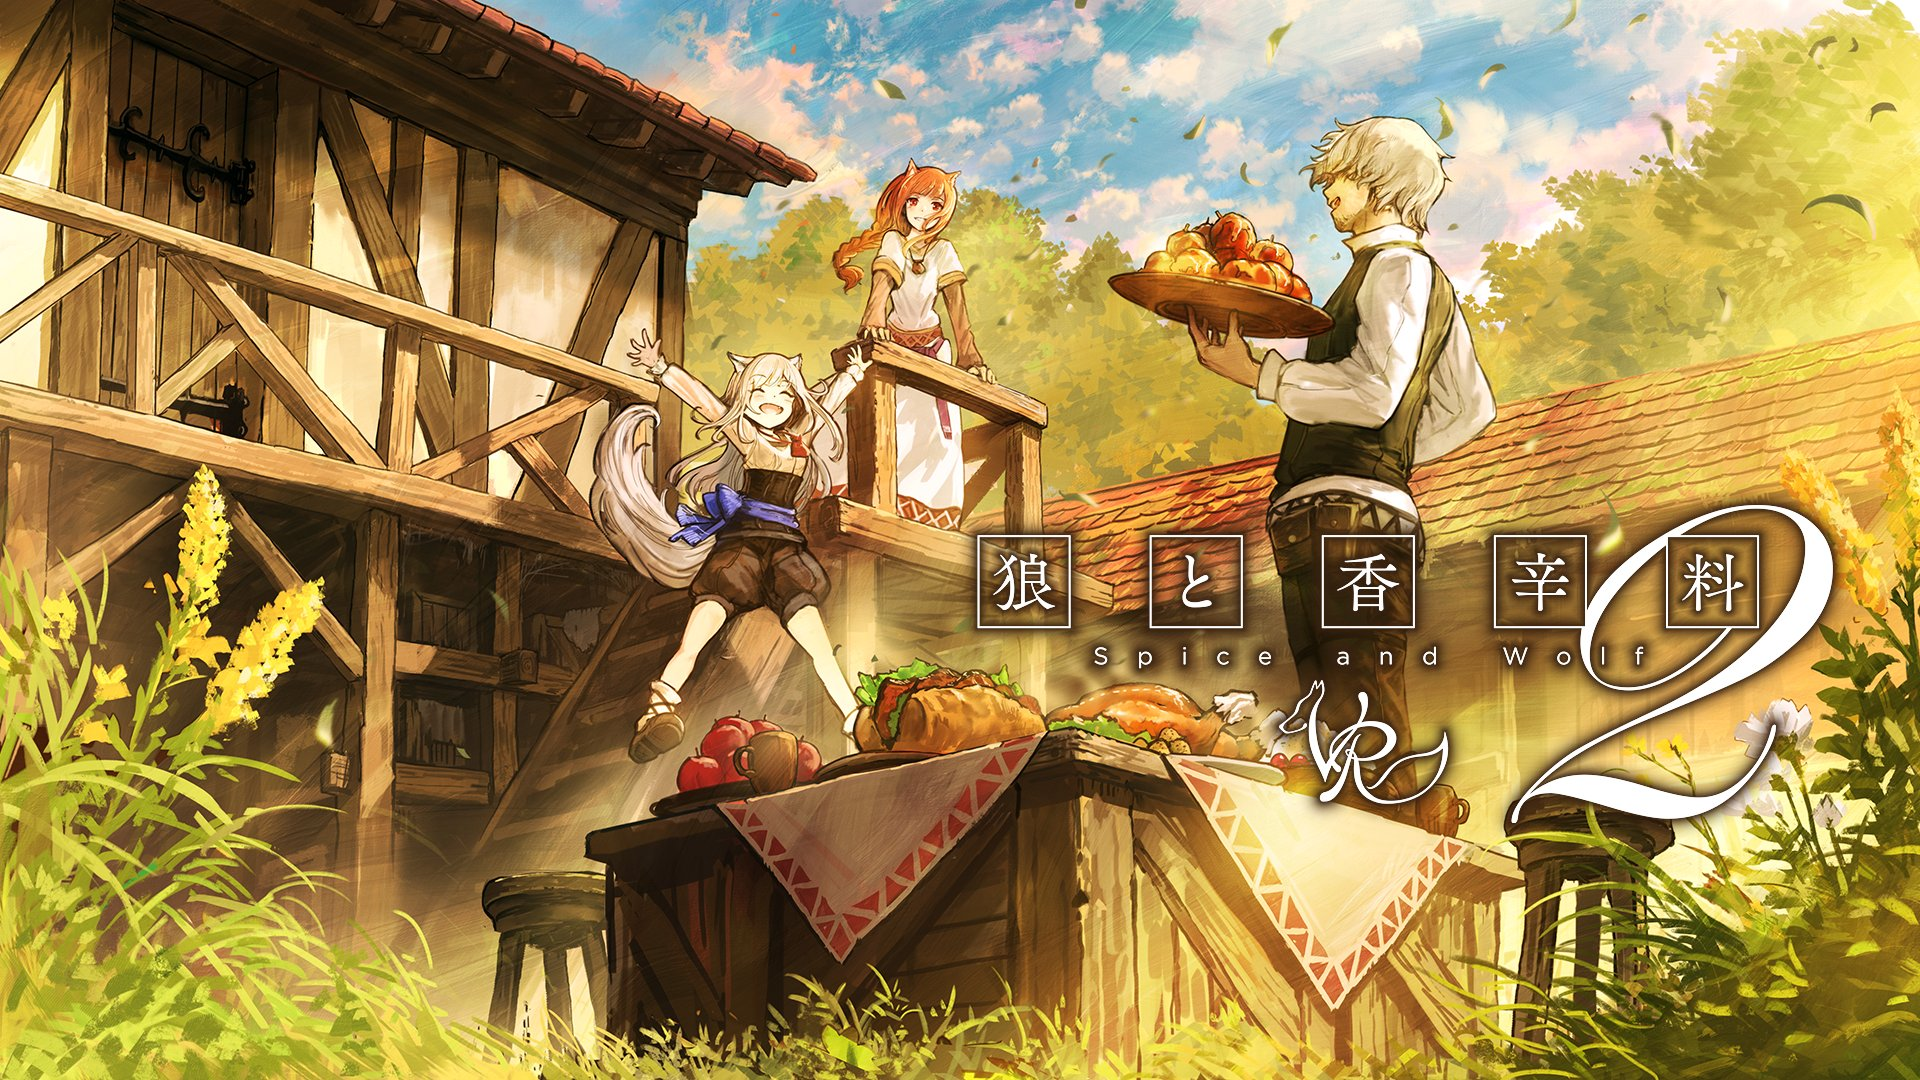
\includegraphics{EisJLXFVkAAZN1c.jpg}

\hypertarget{carga-de-libreruxedas-y-archivos}{%
\section{\texorpdfstring{\textbf{Carga de librerías y
archivos}}{Carga de librerías y archivos}}\label{carga-de-libreruxedas-y-archivos}}

\begin{center}\rule{0.5\linewidth}{0.5pt}\end{center}

Para la obtención del texto de las novelas se realizó la transcripción
de las 23 novelas ligeras a archivos de texto. Junto a estos archivos de
texto se realizó la carga de los léxicos (o lexicon en inglés) para
realizar el análisis de sentimientos. Además, para este trabajo se
necesitó herramientas de text mining, manipulación de dataframes, entre
otros, especificados a continuación:

\begin{Shaded}
\begin{Highlighting}[]
\CommentTok{#Se cargan las librerías}
\KeywordTok{library}\NormalTok{(tidyverse) }\CommentTok{#Manipulación de datos}
\KeywordTok{library}\NormalTok{(tm) }\CommentTok{#Text mining}
\KeywordTok{library}\NormalTok{(wordcloud) }\CommentTok{#Generador de nube de palabras}
\KeywordTok{library}\NormalTok{(wordcloud2) }\CommentTok{#Generador de nube de palabras}
\KeywordTok{library}\NormalTok{(tidytext) }\CommentTok{#Text mining y procesado de palabras}
\KeywordTok{library}\NormalTok{(reshape2) }\CommentTok{#Modificación a dataframes}
\KeywordTok{library}\NormalTok{(RWeka) }\CommentTok{#Data Mining y tokenizador}
\KeywordTok{library}\NormalTok{(knitr) }\CommentTok{#Generación de markdowns}
\KeywordTok{library}\NormalTok{(readtext) }\CommentTok{#Para la lectura de los txt}
\KeywordTok{library}\NormalTok{(kableExtra)}


\CommentTok{#Se cargan los archivos}
\NormalTok{FILEDIR =}\StringTok{ "data_holo/PDF/"}
\NormalTok{filenames <-}\StringTok{ }\KeywordTok{list.files}\NormalTok{(FILEDIR)}
\NormalTok{filenames <-}\StringTok{ }\KeywordTok{gsub}\NormalTok{(}\StringTok{".txt$"}\NormalTok{, }\StringTok{""}\NormalTok{, filenames)}
\NormalTok{txts <-}\StringTok{ }\KeywordTok{readtext}\NormalTok{(FILEDIR)}

\CommentTok{#Se cargan los léxicos para el análisis de sentimiento}
\NormalTok{bing <-}\StringTok{ }\KeywordTok{read_csv}\NormalTok{(}\StringTok{"data/lexi/Bing.csv"}\NormalTok{)}
\NormalTok{nrc <-}\StringTok{ }\KeywordTok{read_csv}\NormalTok{(}\StringTok{"data/lexi/NRC.csv"}\NormalTok{)}
\NormalTok{afinn <-}\StringTok{ }\KeywordTok{read_csv}\NormalTok{(}\StringTok{"data/lexi/Afinn.csv"}\NormalTok{)}
\end{Highlighting}
\end{Shaded}

\hypertarget{preprocesado-de-las-novelas}{%
\section{\texorpdfstring{\textbf{Preprocesado de las
novelas}}{Preprocesado de las novelas}}\label{preprocesado-de-las-novelas}}

\begin{center}\rule{0.5\linewidth}{0.5pt}\end{center}

Antes de realizar cualquier análisis es necesario ordenar las columnas
según su orden de publicación. Además se debe limpiar el texto para
poder utilizarlo. La limpieza consistirá en eliminar carácteres
extraños, tabulaciones, espacios, saltos de línea, números, juntar
palabras, eliminar stopwords y puntuaciones.

\begin{Shaded}
\begin{Highlighting}[]
\CommentTok{#Se crea el orden de las novelas para crear transformar las variables a factor ordenado}
\NormalTok{order_levels <-}\StringTok{ }\KeywordTok{c}\NormalTok{(}\StringTok{"Spice and Wolf  Vol1"}\NormalTok{,}\StringTok{"Spice and Wolf  Vol2"}\NormalTok{,}\StringTok{"Spice and Wolf  Vol3"}\NormalTok{,}
                  \StringTok{"Spice and Wolf  Vol4"}\NormalTok{,}\StringTok{"Spice and Wolf  Vol5"}\NormalTok{,}\StringTok{"Spice and Wolf  Vol6"}\NormalTok{,}
                  \StringTok{"Spice and Wolf  Vol7"}\NormalTok{,}\StringTok{"Spice and Wolf  Vol8"}\NormalTok{,}\StringTok{"Spice and Wolf  Vol9"}\NormalTok{,}
                  \StringTok{"Spice and Wolf  Vol10"}\NormalTok{,}\StringTok{"Spice and Wolf  Vol11"}\NormalTok{,}\StringTok{"Spice and Wolf  Vol12"}\NormalTok{,}
                  \StringTok{"Spice and Wolf  Vol13"}\NormalTok{,}\StringTok{"Spice and Wolf  Vol14"}\NormalTok{,}\StringTok{"Spice and Wolf  Vol15"}\NormalTok{,}
                  \StringTok{"Spice and Wolf  Vol16"}\NormalTok{,}\StringTok{"Spice and Wolf  Vol17"}\NormalTok{,}\StringTok{"Spice and Wolf  Vol18"}\NormalTok{,}
                  \StringTok{"Spice and Wolf  Vol19"}\NormalTok{,}\StringTok{"Spice and Wolf  Vol20"}\NormalTok{,}\StringTok{"Spice and Wolf  Vol21"}\NormalTok{,}
                  \StringTok{"Spice and Wolf s2 Vol1"}\NormalTok{,}\StringTok{"Spice and Wolf s2 Vol2"}
\NormalTok{                  )}
\CommentTok{#Se cambia el tipo de columna con los nombres a factor}
\NormalTok{txts}\OperatorTok{$}\NormalTok{doc_id <-}\StringTok{ }\KeywordTok{factor}\NormalTok{(txts}\OperatorTok{$}\NormalTok{doc_id, }\DataTypeTok{levels =}\NormalTok{ order_levels)}


\CommentTok{#Se crea una función para eliminar el caracter 's expresado en el código de lectura como ’s}
\NormalTok{tryfunc <-}\StringTok{ }\ControlFlowTok{function}\NormalTok{(x) }\KeywordTok{gsub}\NormalTok{(}\StringTok{"’s"}\NormalTok{, }\StringTok{""}\NormalTok{, x)}
\CommentTok{#Limpieza del texto, se remueven todos los carácteres que no se quieren }
\CommentTok{#utilizar y se corrige separaciones erroneas con la función CleanCorpus}

\NormalTok{cleanCorpus <-}\StringTok{ }\ControlFlowTok{function}\NormalTok{(corpus)\{}
  \CommentTok{#Para realizar la limpieza la entrada tiene que estar en formato corpus}
\NormalTok{  s.cor <-}\StringTok{ }\KeywordTok{Corpus}\NormalTok{(}\KeywordTok{VectorSource}\NormalTok{(corpus))}
\NormalTok{  corpus.tmp <-}\StringTok{ }\KeywordTok{tm_map}\NormalTok{(s.cor, }\ControlFlowTok{function}\NormalTok{(x) }\KeywordTok{gsub}\NormalTok{(}\StringTok{"}\CharTok{\textbackslash{}\textbackslash{}}\StringTok{t"}\NormalTok{, }\StringTok{" "}\NormalTok{, x)) }\CommentTok{#Eliminar tabulaciones}
\NormalTok{  corpus.tmp <-}\StringTok{ }\KeywordTok{tm_map}\NormalTok{(corpus.tmp, }\ControlFlowTok{function}\NormalTok{(x) }\KeywordTok{gsub}\NormalTok{(}\StringTok{"}\CharTok{\textbackslash{}\textbackslash{}}\StringTok{n"}\NormalTok{, }\StringTok{" "}\NormalTok{, x)) }\CommentTok{#Eliminar saltos de línea}
\NormalTok{  corpus.tmp <-}\StringTok{ }\KeywordTok{tm_map}\NormalTok{(corpus.tmp, }\ControlFlowTok{function}\NormalTok{(x) }\KeywordTok{gsub}\NormalTok{(}\StringTok{"—"}\NormalTok{, }\StringTok{" "}\NormalTok{, x)) }\CommentTok{#Eliminar doble -- unido}
\NormalTok{  corpus.tmp <-}\StringTok{ }\KeywordTok{tm_map}\NormalTok{(corpus.tmp, }\ControlFlowTok{function}\NormalTok{(x) }\KeywordTok{gsub}\NormalTok{(}\StringTok{"-"}\NormalTok{, }\StringTok{""}\NormalTok{, x)) }\CommentTok{#Eliminar  -}

\NormalTok{  corpus.tmp <-}\StringTok{ }\KeywordTok{tm_map}\NormalTok{(corpus.tmp, removePunctuation) }\CommentTok{#Remover puntuaciones}
\NormalTok{  corpus.tmp <-}\StringTok{ }\KeywordTok{tm_map}\NormalTok{(corpus.tmp, stripWhitespace) }\CommentTok{#Remover espacios}
\NormalTok{  corpus.tmp <-}\StringTok{ }\KeywordTok{tm_map}\NormalTok{(corpus.tmp, }\KeywordTok{content_transformer}\NormalTok{(tolower)) }\CommentTok{#Dejar en minúscula}
\NormalTok{  v_stopwords <-}\StringTok{ }\KeywordTok{c}\NormalTok{(}\KeywordTok{stopwords}\NormalTok{(}\StringTok{"english"}\NormalTok{), }\KeywordTok{c}\NormalTok{(}\StringTok{"thats"}\NormalTok{,}\StringTok{"weve"}\NormalTok{,}\StringTok{"hes"}\NormalTok{,}\StringTok{"theres"}\NormalTok{,}\StringTok{"ive"}\NormalTok{,}\StringTok{"im"}\NormalTok{,}
                                           \StringTok{"will"}\NormalTok{,}\StringTok{"can"}\NormalTok{,}\StringTok{"cant"}\NormalTok{,}\StringTok{"dont"}\NormalTok{,}\StringTok{"youve"}\NormalTok{,}\StringTok{"us"}\NormalTok{,}
                                           \StringTok{"youre"}\NormalTok{,}\StringTok{"youll"}\NormalTok{,}\StringTok{"theyre"}\NormalTok{,}\StringTok{"whats"}\NormalTok{,}\StringTok{"didnt"}\NormalTok{,}
                                           \StringTok{"chapter"}\NormalTok{,}\StringTok{"p"}\NormalTok{,}\StringTok{"g"}\NormalTok{,}\StringTok{"e"}\NormalTok{,}\StringTok{"like"}\NormalTok{)) }
\NormalTok{  corpus.tmp <-}\StringTok{ }\KeywordTok{tm_map}\NormalTok{(corpus.tmp, removeNumbers) }\CommentTok{#Eliminar números}
\NormalTok{  corpus.tmp <-}\StringTok{ }\KeywordTok{tm_map}\NormalTok{(corpus.tmp, PlainTextDocument) }\CommentTok{#Dejar texto plano}
  \CommentTok{#Eliminar stopwords y otras palabras}
\NormalTok{  corpus.tmp <-}\StringTok{ }\KeywordTok{tm_map}\NormalTok{(corpus.tmp, removeWords, v_stopwords) }
  \CommentTok{#Remplaza el nombre le'roi a leroi}
\NormalTok{  corpus.tmp <-}\StringTok{ }\KeywordTok{tm_map}\NormalTok{(corpus.tmp, }\ControlFlowTok{function}\NormalTok{(x) }\KeywordTok{gsub}\NormalTok{(}\StringTok{"le roi"}\NormalTok{, }\StringTok{"leroi"}\NormalTok{, x)) }
  \CommentTok{#Separación erronea "com pany"}
\NormalTok{  corpus.tmp <-}\StringTok{ }\KeywordTok{tm_map}\NormalTok{(corpus.tmp, }\ControlFlowTok{function}\NormalTok{(x) }\KeywordTok{gsub}\NormalTok{(}\StringTok{"com pany"}\NormalTok{, }\StringTok{"company"}\NormalTok{, x))}
  \CommentTok{#Separación erronea "kie man"}
\NormalTok{  corpus.tmp <-}\StringTok{ }\KeywordTok{tm_map}\NormalTok{(corpus.tmp, }\ControlFlowTok{function}\NormalTok{(x) }\KeywordTok{gsub}\NormalTok{(}\StringTok{"kie man"}\NormalTok{, }\StringTok{"kieman"}\NormalTok{, x))}
  \CommentTok{#Separación erronea "kie man"}
\NormalTok{  corpus.tmp <-}\StringTok{ }\KeywordTok{tm_map}\NormalTok{(corpus.tmp, }\ControlFlowTok{function}\NormalTok{(x) }\KeywordTok{gsub}\NormalTok{(}\StringTok{"mil ton"}\NormalTok{, }\StringTok{"milton"}\NormalTok{, x)) }
  \CommentTok{#Separación erronea "mer cenary"}
\NormalTok{  corpus.tmp <-}\StringTok{ }\KeywordTok{tm_map}\NormalTok{(corpus.tmp, }\ControlFlowTok{function}\NormalTok{(x) }\KeywordTok{gsub}\NormalTok{(}\StringTok{"mer cenary"}\NormalTok{, }\StringTok{"mercenary"}\NormalTok{, x)) }
  \KeywordTok{return}\NormalTok{(corpus.tmp[[}\DecValTok{1}\NormalTok{]][}\DecValTok{1}\NormalTok{])\} }\CommentTok{#Retorna el array dentro del corpus creado}

\CommentTok{#Se crean dos bucles. El primero elimina el caracter 's}
\ControlFlowTok{for}\NormalTok{(i }\ControlFlowTok{in} \DecValTok{1}\OperatorTok{:}\KeywordTok{length}\NormalTok{(txts}\OperatorTok{$}\NormalTok{doc_id))\{}
\NormalTok{  txts[i,}\DecValTok{2}\NormalTok{] <-}\StringTok{ }\KeywordTok{tryfunc}\NormalTok{(txts[i,}\DecValTok{2}\NormalTok{])}
\NormalTok{\}}

\CommentTok{#Luego se intercambia la codificación para que aparezcan las tabulaciones y saltos}
\CommentTok{#como \textbackslash{}t y \textbackslash{}n}
\NormalTok{txts}\OperatorTok{$}\NormalTok{text<-}\StringTok{ }\KeywordTok{iconv}\NormalTok{(txts}\OperatorTok{$}\NormalTok{text, }\StringTok{'utf-8'}\NormalTok{, }\StringTok{'ascii'}\NormalTok{, }\DataTypeTok{sub=}\StringTok{''}\NormalTok{)}

\CommentTok{#El segundo bucle aplica la función cleanCorpus}
\ControlFlowTok{for}\NormalTok{(i }\ControlFlowTok{in} \DecValTok{1}\OperatorTok{:}\KeywordTok{length}\NormalTok{(txts}\OperatorTok{$}\NormalTok{doc_id))\{}
\NormalTok{  txts[i,}\DecValTok{2}\NormalTok{] <-}\StringTok{ }\KeywordTok{cleanCorpus}\NormalTok{(txts[i,}\DecValTok{2}\NormalTok{])}
\NormalTok{\}}

\CommentTok{#Se ordena el dataframe según el factor creado}
\NormalTok{txts <-}\StringTok{ }\NormalTok{txts }\OperatorTok\StringTok{ }\KeywordTok{arrange}\NormalTok{(doc_id)}
\end{Highlighting}
\end{Shaded}

\hypertarget{analisis-de-los-datos}{%
\section{\texorpdfstring{\textbf{Analisis de los
datos}}{Analisis de los datos}}\label{analisis-de-los-datos}}

\begin{center}\rule{0.5\linewidth}{0.5pt}\end{center}

El analisis se separa en la creación de wordclouds, separación entre
palabras según el sentimiento y análisis de monogramas, bigramas y
trigramas.

\hypertarget{nube-de-palabras-seguxfan-su-frecuencia}{%
\subsection{\texorpdfstring{\textbf{Nube de palabras según su
frecuencia}}{Nube de palabras según su frecuencia}}\label{nube-de-palabras-seguxfan-su-frecuencia}}

\begin{center}\rule{0.5\linewidth}{0.5pt}\end{center}

Una forma visual de comenzar el análisis es realizar una nube de
palabras donde el tamaño de las palabras depende de la frecuencia de
aparición en el texto. Por problemas con la librería se realizó una
captura del wordcloud y se publicó como imagen.

\begin{Shaded}
\begin{Highlighting}[]
\CommentTok{#Se crea otra función CleanCorpus2 para poder ser utilizada en la siguiente función}
\NormalTok{cleanCorpus2 <-}\StringTok{ }\ControlFlowTok{function}\NormalTok{(corpus)\{}
\NormalTok{  corpus.tmp <-}\StringTok{ }\KeywordTok{tm_map}\NormalTok{(corpus, removePunctuation)}
\NormalTok{  corpus.tmp <-}\StringTok{ }\KeywordTok{tm_map}\NormalTok{(corpus.tmp, stripWhitespace)}
\NormalTok{  corpus.tmp <-}\StringTok{ }\KeywordTok{tm_map}\NormalTok{(corpus.tmp, }\KeywordTok{content_transformer}\NormalTok{(tolower))}
\NormalTok{  v_stopwords <-}\StringTok{ }\KeywordTok{c}\NormalTok{(}\KeywordTok{stopwords}\NormalTok{(}\StringTok{"english"}\NormalTok{), }\KeywordTok{c}\NormalTok{(}\StringTok{"thats"}\NormalTok{,}\StringTok{"weve"}\NormalTok{,}\StringTok{"hes"}\NormalTok{,}\StringTok{"theres"}\NormalTok{,}\StringTok{"ive"}\NormalTok{,}\StringTok{"im"}\NormalTok{,}
                                           \StringTok{"will"}\NormalTok{,}\StringTok{"can"}\NormalTok{,}\StringTok{"cant"}\NormalTok{,}\StringTok{"dont"}\NormalTok{,}\StringTok{"youve"}\NormalTok{,}\StringTok{"us"}\NormalTok{,}
                                           \StringTok{"youre"}\NormalTok{,}\StringTok{"youll"}\NormalTok{,}\StringTok{"theyre"}\NormalTok{,}\StringTok{"whats"}\NormalTok{,}\StringTok{"didnt"}\NormalTok{, }\StringTok{"like"}\NormalTok{))}
\NormalTok{  corpus.tmp <-}\StringTok{ }\KeywordTok{tm_map}\NormalTok{(corpus.tmp, removeWords, v_stopwords)}
  \KeywordTok{return}\NormalTok{(corpus.tmp)}
  
\NormalTok{\}}

\CommentTok{# Se crea una función para realizar el conteo de palabras}
\NormalTok{frequentTerms <-}\StringTok{ }\ControlFlowTok{function}\NormalTok{(text)\{}
  \CommentTok{#La funcion Corpus del paquete tm crea  y computa el corpus}
  \CommentTok{#Mientras que la función VectorSource interpreta cada elemento de }
  \CommentTok{#text como un documento}
\NormalTok{  s.cor <-}\StringTok{ }\KeywordTok{Corpus}\NormalTok{(}\KeywordTok{VectorSource}\NormalTok{(text))}
  \CommentTok{#Se aplica la primera función creada cleanCorpus2}
\NormalTok{  s.cor.cl <-}\StringTok{ }\KeywordTok{cleanCorpus2}\NormalTok{(s.cor)}
  \CommentTok{#Del paquete tm transforma el documento a una matriz}
\NormalTok{  s.tdm <-}\StringTok{ }\KeywordTok{TermDocumentMatrix}\NormalTok{(s.cor.cl)}
  \CommentTok{#Remueve elementos que aparecen en pequeñas cantidades}
\NormalTok{  s.tdm <-}\StringTok{ }\KeywordTok{removeSparseTerms}\NormalTok{(s.tdm, }\FloatTok{0.999}\NormalTok{)}
  \CommentTok{#Transforma los datos a una matriz de R}
\NormalTok{  m <-}\StringTok{ }\KeywordTok{as.matrix}\NormalTok{(s.tdm)}
  \CommentTok{#Se suma por fila para obtener la frecuencia}
  \CommentTok{#Como está ordenado como matriz se ordena según la frecuencia más alta}
\NormalTok{  word_freqs <-}\StringTok{ }\KeywordTok{sort}\NormalTok{(}\KeywordTok{rowSums}\NormalTok{(m), }\DataTypeTok{decreasing=}\OtherTok{TRUE}\NormalTok{)}
  \CommentTok{#Se crea un dataframe con estas frecuencias}
\NormalTok{  dm <-}\StringTok{ }\KeywordTok{data.frame}\NormalTok{(}\DataTypeTok{word=}\KeywordTok{names}\NormalTok{(word_freqs), }\DataTypeTok{freq=}\NormalTok{word_freqs)}
  \KeywordTok{return}\NormalTok{(dm)}
  
\NormalTok{\}}

\CommentTok{#wordcloud2 tiene problemas al crear las nubes cuando palabras destacan mucho por }
\CommentTok{#sobre otras, por lo cual se le asignó un valor más adecuado.}
\NormalTok{jj <-}\StringTok{ }\KeywordTok{frequentTerms}\NormalTok{(txts}\OperatorTok{$}\NormalTok{text)}
\NormalTok{jj[}\DecValTok{1}\NormalTok{,}\DecValTok{2}\NormalTok{] =}\StringTok{ }\DecValTok{7000}
\NormalTok{jj[}\DecValTok{2}\NormalTok{,}\DecValTok{2}\NormalTok{] =}\StringTok{ }\DecValTok{6000}

\NormalTok{hw =}\StringTok{ }\KeywordTok{wordcloud2}\NormalTok{(jj, }\DataTypeTok{size=}\DecValTok{3}\NormalTok{, }\DataTypeTok{figPath =}\StringTok{"../Imagen4.png"}\NormalTok{)}
\end{Highlighting}
\end{Shaded}

Se puede observar que las palabras que más aparecen es Holo y Lawrence,
protagonistas de la serie.

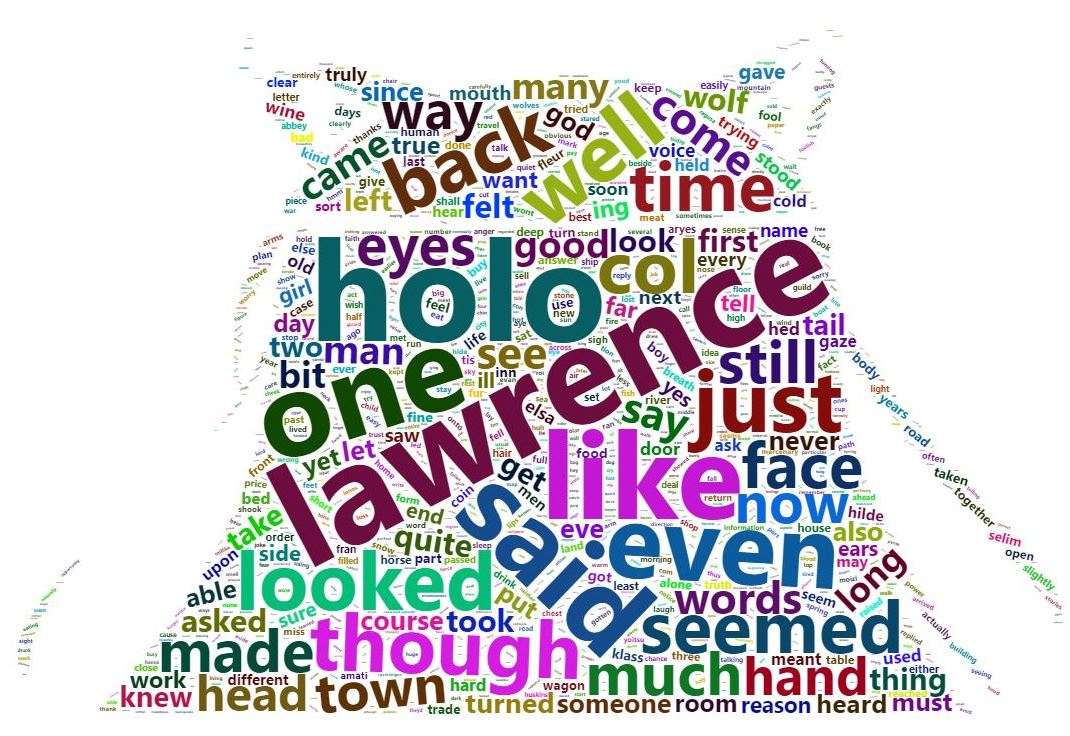
\includegraphics{descarga2.jpg}

\begin{figure}
\centering
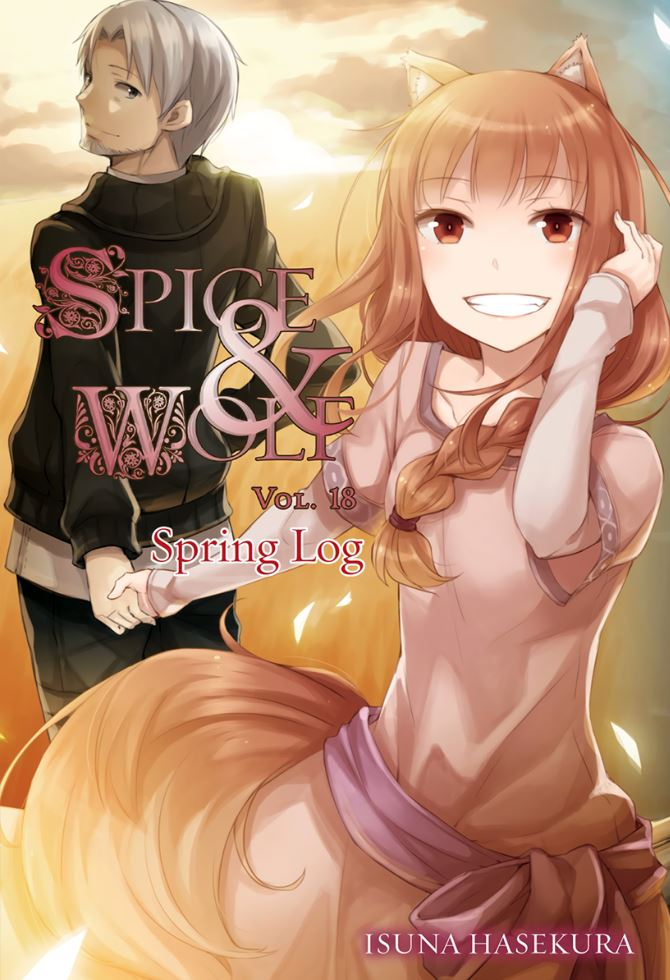
\includegraphics[width=3.85417in,height=\textheight]{Capturaholo.jpg}
\caption{Spice and Wolf: Lawrence y Holo}
\end{figure}

\hypertarget{nube-de-palabras-seguxfan-luxe9xico-bing}{%
\subsection{\texorpdfstring{\textbf{Nube de palabras según léxico
Bing}}{Nube de palabras según léxico Bing}}\label{nube-de-palabras-seguxfan-luxe9xico-bing}}

\begin{center}\rule{0.5\linewidth}{0.5pt}\end{center}

A continuación se realizó el wordcloud de las palabras separadas según
el léxico genérico de bing, de
\href{https://www.cs.uic.edu/~liub/FBS/sentiment-analysis.html}{Bing Liu
y colaboradores} que separó palabras según negativas y positivas. El
léxico bing se ve de la siguiente manera: `

\begin{table}[H]
\centering
\begin{tabular}[t]{l|l}
\hline
word & sentiment\\
\hline
obstructed & negative\\
\hline
obstructing & negative\\
\hline
obstruction & negative\\
\hline
obstructs & negative\\
\hline
obtainable & positive\\
\hline
obtrusive & negative\\
\hline
\end{tabular}
\end{table}

Se observa que el léxico bing separa las palabras en positivas y
negativas.

\begin{Shaded}
\begin{Highlighting}[]
\CommentTok{#Tokeniza el texto de las novelas}
\NormalTok{tokens <-}\StringTok{ }\NormalTok{txts }\OperatorTok\StringTok{  }
\StringTok{  }\KeywordTok{mutate}\NormalTok{(}\DataTypeTok{text=}\KeywordTok{as.character}\NormalTok{(txts}\OperatorTok{$}\NormalTok{text)) }\OperatorTok
\StringTok{  }\KeywordTok{unnest_tokens}\NormalTok{(word, text)}

\NormalTok{tokens }\OperatorTok
\StringTok{  }\KeywordTok{inner_join}\NormalTok{(}\KeywordTok{get_sentiments}\NormalTok{(}\StringTok{"bing"}\NormalTok{)) }\OperatorTok\StringTok{ }\CommentTok{#Se agrega si son palabras positivas o negativas}
\StringTok{  }\KeywordTok{count}\NormalTok{(word, sentiment, }\DataTypeTok{sort=}\OtherTok{TRUE}\NormalTok{) }\OperatorTok\StringTok{ }\CommentTok{#Se realiza el conteo de las palabras}
\StringTok{  }\KeywordTok{acast}\NormalTok{(word }\OperatorTok{~}\StringTok{ }\NormalTok{sentiment, }\DataTypeTok{value.var=}\StringTok{"n"}\NormalTok{, }\DataTypeTok{fill=}\DecValTok{0}\NormalTok{) }\OperatorTok\StringTok{ }\CommentTok{#Separa en positivo o negativo}
\StringTok{  }\KeywordTok{comparison.cloud}\NormalTok{(}\DataTypeTok{colors=}\KeywordTok{c}\NormalTok{(}\StringTok{"#3399FF"}\NormalTok{, }\StringTok{"#CC6600"}\NormalTok{), }\DataTypeTok{max.words=}\DecValTok{300}\NormalTok{, }\DataTypeTok{title.size =} \DecValTok{2}\NormalTok{, }
                   \DataTypeTok{title.colors =} \KeywordTok{c}\NormalTok{(}\StringTok{"#3399FF"}\NormalTok{, }\StringTok{"#CC6600"}\NormalTok{)) }\CommentTok{#Se crea la nube de palabras}
\end{Highlighting}
\end{Shaded}

\begin{center}\includegraphics{Tarea1_files/figure-latex/unnamed-chunk-5-1} \end{center}

\hypertarget{anuxe1lisis-de-sentimiento-utilizando-el-luxe9xico-nrc}{%
\subsection{\texorpdfstring{\textbf{Análisis de sentimiento utilizando
el léxico
NRC}}{Análisis de sentimiento utilizando el léxico NRC}}\label{anuxe1lisis-de-sentimiento-utilizando-el-luxe9xico-nrc}}

\begin{center}\rule{0.5\linewidth}{0.5pt}\end{center}

El siguiente análisis utiliza el lexicon NRC, de
\href{http://saifmohammad.com/WebPages/NRC-Emotion-Lexicon.htm}{Saif
Mohammad y Peter Turney}, el cual no solo contiene la denominación de
las palabras como positivo y negativo, contiene sentimientos (o
emociones) de verdad, anticipación, sorpresa, enojo, entre otros. Este
análisis se realizará considerando todas las novelas en su conjunto. El
léxico NRC se ve de la siguiente manera:

\begin{table}[H]
\centering
\begin{tabular}[t]{l|l}
\hline
word & sentiment\\
\hline
lofty & negative\\
\hline
logical & positive\\
\hline
lone & sadness\\
\hline
loneliness & fear\\
\hline
loneliness & negative\\
\hline
loneliness & sadness\\
\hline
\end{tabular}
\end{table}

Se observa que el léxico NRC contiene palabras separadas como positivas,
negativas, pero además otras como miedo, tristeza, entre otras
emociones. Con el léxico se realizó el conteo de palabras
correspondientes a los sentimientos y emociones del universo de las
novelas.

\begin{Shaded}
\begin{Highlighting}[]
\CommentTok{#Se crea una paleta de colores para el gráfico}
\NormalTok{palette1 =}\StringTok{ }\KeywordTok{c}\NormalTok{(}\StringTok{"#f4d9b8"}\NormalTok{, }\StringTok{"#daa688"}\NormalTok{, }\StringTok{"#f3e5d4"}\NormalTok{, }\StringTok{"#f3cd9c"}\NormalTok{, }
             \StringTok{"#e3beaa"}\NormalTok{, }\StringTok{"#c17646"}\NormalTok{, }\StringTok{"#b35e25"}\NormalTok{, }\StringTok{"#f4d3aa"}\NormalTok{, }\StringTok{"#f4dfc6"}\NormalTok{, }\StringTok{"#ce8e66"}\NormalTok{ )}

\CommentTok{# Sentimientos y frecuencia asociada a cada palabra }
\NormalTok{sentiments <-}\StringTok{ }\NormalTok{tokens }\OperatorTok\StringTok{ }
\StringTok{  }\KeywordTok{inner_join}\NormalTok{(nrc, }\StringTok{"word"}\NormalTok{) }\OperatorTok
\StringTok{  }\KeywordTok{count}\NormalTok{(word, sentiment, }\DataTypeTok{sort=}\OtherTok{TRUE}\NormalTok{) }


\CommentTok{# Grárico de frecuencia de cada sentimiento}
\KeywordTok{ggplot}\NormalTok{(}\DataTypeTok{data=}\NormalTok{sentiments, }\KeywordTok{aes}\NormalTok{(}\DataTypeTok{x=}\KeywordTok{reorder}\NormalTok{(sentiment, }\OperatorTok{-}\NormalTok{n, sum), }\DataTypeTok{y=}\NormalTok{n)) }\OperatorTok{+}\StringTok{ }
\StringTok{  }\KeywordTok{geom_bar}\NormalTok{(}\DataTypeTok{stat=}\StringTok{"identity"}\NormalTok{, }\KeywordTok{aes}\NormalTok{(}\DataTypeTok{fill=}\NormalTok{sentiment), }\DataTypeTok{show.legend=}\OtherTok{FALSE}\NormalTok{) }\OperatorTok{+}
\StringTok{  }\KeywordTok{scale_fill_manual}\NormalTok{(}\DataTypeTok{values=}\NormalTok{palette1) }\OperatorTok{+}
\StringTok{  }\KeywordTok{labs}\NormalTok{(}\DataTypeTok{x=}\StringTok{"Sentimiento"}\NormalTok{, }\DataTypeTok{y=}\StringTok{"Frecuencia"}\NormalTok{) }\OperatorTok{+}
\StringTok{  }\KeywordTok{ggtitle}\NormalTok{(}\StringTok{"Frecuencia según el sentimiento de léxico NRC"}\NormalTok{) }\OperatorTok{+}
\StringTok{  }\KeywordTok{theme_bw}\NormalTok{() }\OperatorTok{+}
\StringTok{  }\KeywordTok{theme}\NormalTok{(}\DataTypeTok{plot.title =} \KeywordTok{element_text}\NormalTok{(}\DataTypeTok{hjust =} \FloatTok{0.5}\NormalTok{))}
\end{Highlighting}
\end{Shaded}

\includegraphics[width=1.5\linewidth,height=1.5\textheight]{Tarea1_files/figure-latex/unnamed-chunk-7-1}

Se puede observar que el sentimiento que predomina es el positivo sobre
el negativo. Además de sentimientos como verdad y anticipación, debido a
que es una novela de una pareja de comerciantes, es más que esperable
que aparezcan.

\hypertarget{palabras-muxe1s-frecuentes-seguxfan-el-sentimiento-usando-luxe9xico-nrc}{%
\subsubsection{\texorpdfstring{\textbf{Palabras más frecuentes según el
sentimiento usando léxico
NRC}}{Palabras más frecuentes según el sentimiento usando léxico NRC}}\label{palabras-muxe1s-frecuentes-seguxfan-el-sentimiento-usando-luxe9xico-nrc}}

Se realizó el análisis de palabras más frecuentes según el sentimiento,
considerando todas las novelas en su conjunto

\begin{Shaded}
\begin{Highlighting}[]
\NormalTok{palette =}\StringTok{ }\KeywordTok{c}\NormalTok{(}\StringTok{"#fcc082"}\NormalTok{,}\StringTok{"#d68128"}\NormalTok{,}\StringTok{"#d68128"}\NormalTok{,}\StringTok{"#d68128"}\NormalTok{,}\StringTok{"#d68128"}\NormalTok{,}\StringTok{"#e1a35f"}\NormalTok{,}
            \StringTok{"#e1a35f"}\NormalTok{,}\StringTok{"#e1a35f"}\NormalTok{,}\StringTok{"#e1a35f"}\NormalTok{,}\StringTok{"#fcc082"}\NormalTok{,}\StringTok{"#fcc082"}\NormalTok{,}\StringTok{"#fcc082"}\NormalTok{)}
\NormalTok{sentiments }\OperatorTok
\StringTok{  }\KeywordTok{group_by}\NormalTok{(sentiment) }\OperatorTok
\StringTok{  }\KeywordTok{arrange}\NormalTok{(}\KeywordTok{desc}\NormalTok{(n)) }\OperatorTok
\StringTok{  }\KeywordTok{slice}\NormalTok{(}\DecValTok{1}\OperatorTok{:}\DecValTok{10}\NormalTok{) }\OperatorTok
\StringTok{  }\KeywordTok{ggplot}\NormalTok{(}\KeywordTok{aes}\NormalTok{(}\DataTypeTok{x=}\KeywordTok{reorder}\NormalTok{(word, n), }\DataTypeTok{y=}\NormalTok{n)) }\OperatorTok{+}
\StringTok{  }\KeywordTok{geom_col}\NormalTok{(}\KeywordTok{aes}\NormalTok{(}\DataTypeTok{fill=}\NormalTok{sentiment), }\DataTypeTok{show.legend=}\OtherTok{FALSE}\NormalTok{)  }\OperatorTok{+}
\StringTok{  }\KeywordTok{scale_fill_manual}\NormalTok{(}\DataTypeTok{values=}\NormalTok{palette) }\OperatorTok{+}
\StringTok{  }\KeywordTok{facet_wrap}\NormalTok{(}\OperatorTok{~}\NormalTok{sentiment, }\DataTypeTok{scales=}\StringTok{"free_y"}\NormalTok{) }\OperatorTok{+}
\StringTok{  }\KeywordTok{labs}\NormalTok{(}\DataTypeTok{y=}\StringTok{"Frecuencia"}\NormalTok{, }\DataTypeTok{x=}\StringTok{"Término"}\NormalTok{) }\OperatorTok{+}
\StringTok{  }\KeywordTok{coord_flip}\NormalTok{() }\OperatorTok{+}
\StringTok{  }\KeywordTok{ggtitle}\NormalTok{(}\StringTok{"Términos más repetidos por sentimiento usando léxico NRC"}\NormalTok{) }\OperatorTok{+}
\StringTok{  }\KeywordTok{theme_bw}\NormalTok{() }\OperatorTok{+}
\StringTok{  }\KeywordTok{theme}\NormalTok{(}\DataTypeTok{plot.title =} \KeywordTok{element_text}\NormalTok{(}\DataTypeTok{hjust =} \FloatTok{0.5}\NormalTok{))}
\end{Highlighting}
\end{Shaded}

\includegraphics[width=1.5\linewidth,height=1.5\textheight]{Tarea1_files/figure-latex/unnamed-chunk-8-1}
Se puede observar que palabras como money, \textbf{ill},
\textbf{church}, \textbf{lie}, \textbf{god} son palabras muy esperadas
para una novela ambientada en el tiempo medieval. En cuanto a los
sentimientos que le corresponde a cada palabra son esperables,
\textbf{ill} (enfermo), representa enojo, disgusto, miedo, tristeza;
\textbf{money} (moneda) representa anticipación, enojo, alegría,
positivo, sorpresa, confianza. Con esto nos damos cuenta que es muy
dificil para el código contextualizar las palabras, aunque nos ayuda a
tener una idea general del problema.

\hypertarget{sentimientos-muxe1s-frecuentes-seguxfan-la-novela-usando-luxe9xico-nrc}{%
\subsubsection{\texorpdfstring{\textbf{Sentimientos más frecuentes según
la novela usando léxico
NRC}}{Sentimientos más frecuentes según la novela usando léxico NRC}}\label{sentimientos-muxe1s-frecuentes-seguxfan-la-novela-usando-luxe9xico-nrc}}

Otro análisis que se realizó es el de sentimientos pero por novela
utilizando el léxico NRC. Por temas estéticos los gráficos se separarán
desde la novela 1 a la 12 y de la 13 a la 23

\hypertarget{sentimientos-novelas-1-12}{%
\paragraph{\texorpdfstring{\textbf{Sentimientos Novelas
1-12}}{Sentimientos Novelas 1-12}}\label{sentimientos-novelas-1-12}}

\begin{Shaded}
\begin{Highlighting}[]
\NormalTok{tokens }\OperatorTok
\StringTok{  }\KeywordTok{filter}\NormalTok{(doc_id }\OperatorTok\StringTok{ }\NormalTok{order_levels[}\DecValTok{1}\OperatorTok{:}\DecValTok{12}\NormalTok{]) }\OperatorTok
\StringTok{  }\KeywordTok{inner_join}\NormalTok{(nrc, }\StringTok{"word"}\NormalTok{) }\OperatorTok
\StringTok{  }\KeywordTok{count}\NormalTok{(doc_id, sentiment, }\DataTypeTok{sort=}\OtherTok{TRUE}\NormalTok{) }\OperatorTok
\StringTok{  }\KeywordTok{ggplot}\NormalTok{(}\KeywordTok{aes}\NormalTok{(}\DataTypeTok{x=}\NormalTok{sentiment, }\DataTypeTok{y=}\NormalTok{n)) }\OperatorTok{+}
\StringTok{  }\KeywordTok{geom_col}\NormalTok{(}\KeywordTok{aes}\NormalTok{(}\DataTypeTok{fill=}\NormalTok{doc_id), }\DataTypeTok{show.legend=}\OtherTok{FALSE}\NormalTok{) }\OperatorTok{+}
\StringTok{  }\KeywordTok{scale_fill_manual}\NormalTok{(}\DataTypeTok{values=}\NormalTok{palette) }\OperatorTok{+}
\StringTok{  }\KeywordTok{facet_wrap}\NormalTok{(}\OperatorTok{~}\NormalTok{doc_id, }\DataTypeTok{scales=}\StringTok{"free_y"}\NormalTok{) }\OperatorTok{+}
\StringTok{  }\KeywordTok{labs}\NormalTok{(}\DataTypeTok{x=}\StringTok{"Sentimiento"}\NormalTok{, }\DataTypeTok{y=}\StringTok{"Frecuencia"}\NormalTok{) }\OperatorTok{+}
\StringTok{  }\KeywordTok{coord_flip}\NormalTok{() }\OperatorTok{+}
\StringTok{  }\KeywordTok{ggtitle}\NormalTok{(}\StringTok{"Frecuencia de sentimientos por volumen"}\NormalTok{) }\OperatorTok{+}
\StringTok{  }\KeywordTok{theme_bw}\NormalTok{() }\OperatorTok{+}
\StringTok{  }\KeywordTok{theme}\NormalTok{(}\DataTypeTok{plot.title =} \KeywordTok{element_text}\NormalTok{(}\DataTypeTok{hjust =} \FloatTok{0.5}\NormalTok{))}
\end{Highlighting}
\end{Shaded}

\includegraphics[width=1.5\linewidth,height=1.5\textheight]{Tarea1_files/figure-latex/unnamed-chunk-9-1}

\hypertarget{sentimientos-novelas-13-23}{%
\paragraph{\texorpdfstring{\textbf{Sentimientos Novelas
13-23}}{Sentimientos Novelas 13-23}}\label{sentimientos-novelas-13-23}}

\begin{Shaded}
\begin{Highlighting}[]
\NormalTok{tokens }\OperatorTok
\StringTok{  }\KeywordTok{filter}\NormalTok{(doc_id }\OperatorTok\StringTok{ }\NormalTok{order_levels[}\DecValTok{13}\OperatorTok{:}\DecValTok{23}\NormalTok{]) }\OperatorTok
\StringTok{  }\KeywordTok{inner_join}\NormalTok{(nrc, }\StringTok{"word"}\NormalTok{) }\OperatorTok
\StringTok{  }\KeywordTok{count}\NormalTok{(doc_id, sentiment, }\DataTypeTok{sort=}\OtherTok{TRUE}\NormalTok{) }\OperatorTok
\StringTok{  }\KeywordTok{ggplot}\NormalTok{(}\KeywordTok{aes}\NormalTok{(}\DataTypeTok{y=}\NormalTok{sentiment, }\DataTypeTok{x=}\NormalTok{n)) }\OperatorTok{+}
\StringTok{  }\KeywordTok{geom_col}\NormalTok{(}\KeywordTok{aes}\NormalTok{(}\DataTypeTok{fill=}\NormalTok{doc_id), }\DataTypeTok{show.legend=}\OtherTok{FALSE}\NormalTok{) }\OperatorTok{+}
\StringTok{  }\KeywordTok{facet_wrap}\NormalTok{(}\OperatorTok{~}\NormalTok{doc_id, }\DataTypeTok{scales=}\StringTok{"free_y"}\NormalTok{) }\OperatorTok{+}
\StringTok{  }\KeywordTok{scale_fill_manual}\NormalTok{(}\DataTypeTok{values=}\NormalTok{palette) }\OperatorTok{+}
\StringTok{  }\KeywordTok{labs}\NormalTok{(}\DataTypeTok{x=}\StringTok{"Sentimiento"}\NormalTok{, }\DataTypeTok{y=}\StringTok{"Frecuencia"}\NormalTok{) }\OperatorTok{+}
\StringTok{  }\KeywordTok{ggtitle}\NormalTok{(}\StringTok{"Frecuencia de sentimientos por volumen"}\NormalTok{) }\OperatorTok{+}
\StringTok{  }\KeywordTok{theme_bw}\NormalTok{() }\OperatorTok{+}
\StringTok{  }\KeywordTok{theme}\NormalTok{(}\DataTypeTok{plot.title =} \KeywordTok{element_text}\NormalTok{(}\DataTypeTok{hjust =} \FloatTok{0.5}\NormalTok{))}
\end{Highlighting}
\end{Shaded}

\includegraphics[width=1.5\linewidth,height=1.5\textheight]{Tarea1_files/figure-latex/unnamed-chunk-10-1}

Se puede observar comportamientos muy parecidos entre las novelas.
Exceptuando por el volumen 16 donde el sentimiento negativo sobrepasa el
positivo, lo cual si se sigue la lectura de este volumen es esperable al
encontrarse en un ambiente de guerras entre ciudades.

\hypertarget{anuxe1lisis-de-sentimiento-utilizando-el-luxe9xico-afinn}{%
\subsection{\texorpdfstring{\textbf{Análisis de sentimiento utilizando
el léxico
AFINN}}{Análisis de sentimiento utilizando el léxico AFINN}}\label{anuxe1lisis-de-sentimiento-utilizando-el-luxe9xico-afinn}}

\begin{center}\rule{0.5\linewidth}{0.5pt}\end{center}

Otro léxico que se puede utilizar es el
\href{http://www2.imm.dtu.dk/pubdb/pubs/6010-full.html}{AFINN}, el que
da puntaje según el tipo de palabra. A valores negativos, sentimientos
negativos y vice versa. El siguiente gráfico muestra cuantas palabras
corresponden a cada puntaje. El léxico AFINN se ve de la siguiente
manera:

\begin{table}[H]
\centering
\begin{tabular}[t]{l|r}
\hline
word & value\\
\hline
banned & -2\\
\hline
bargain & 2\\
\hline
barrier & -2\\
\hline
bastard & -5\\
\hline
bastards & -5\\
\hline
battle & -1\\
\hline
\end{tabular}
\end{table}

Se observa que el léxico AFINN entrega valoraciones a las palabras de
que tan positivas y que tan negativas son.

\begin{Shaded}
\begin{Highlighting}[]
\NormalTok{tokens }\OperatorTok\StringTok{ }
\StringTok{  }\KeywordTok{inner_join}\NormalTok{(afinn, }\StringTok{"word"}\NormalTok{) }\OperatorTok\StringTok{ }
\StringTok{  }\KeywordTok{count}\NormalTok{(value, }\DataTypeTok{sort=}\NormalTok{T) }\OperatorTok
\StringTok{  }\KeywordTok{ggplot}\NormalTok{(}\KeywordTok{aes}\NormalTok{(}\DataTypeTok{x=}\NormalTok{value, }\DataTypeTok{y=}\NormalTok{n)) }\OperatorTok{+}
\StringTok{  }\KeywordTok{geom_bar}\NormalTok{(}\DataTypeTok{stat=}\StringTok{"identity"}\NormalTok{, }\KeywordTok{aes}\NormalTok{(}\DataTypeTok{fill=}\NormalTok{n), }\DataTypeTok{show.legend=}\OtherTok{FALSE}\NormalTok{, }\DataTypeTok{width=}\FloatTok{0.5}\NormalTok{) }\OperatorTok{+}
\StringTok{  }\KeywordTok{geom_label}\NormalTok{(}\KeywordTok{aes}\NormalTok{(}\DataTypeTok{label=}\NormalTok{n)) }\OperatorTok{+}
\StringTok{  }\KeywordTok{scale_fill_gradient}\NormalTok{(}\DataTypeTok{low=}\StringTok{"#f3cd9c"}\NormalTok{, }\DataTypeTok{high=}\StringTok{"#b35e25"}\NormalTok{) }\OperatorTok{+}
\StringTok{  }\KeywordTok{scale_x_continuous}\NormalTok{(}\DataTypeTok{breaks=}\KeywordTok{seq}\NormalTok{(}\OperatorTok{-}\DecValTok{5}\NormalTok{, }\DecValTok{5}\NormalTok{, }\DecValTok{1}\NormalTok{)) }\OperatorTok{+}
\StringTok{  }\KeywordTok{labs}\NormalTok{(}\DataTypeTok{x=}\StringTok{"Puntaje"}\NormalTok{, }\DataTypeTok{y=}\StringTok{"Frecuencia"}\NormalTok{) }\OperatorTok{+}
\StringTok{  }\KeywordTok{ggtitle}\NormalTok{(}\StringTok{"Distribución de palabras según el léxico AFINN"}\NormalTok{) }\OperatorTok{+}
\StringTok{  }\KeywordTok{theme_bw}\NormalTok{() }\OperatorTok{+}
\StringTok{  }\KeywordTok{theme}\NormalTok{(}\DataTypeTok{plot.title =} \KeywordTok{element_text}\NormalTok{(}\DataTypeTok{hjust =} \FloatTok{0.5}\NormalTok{)) }
\end{Highlighting}
\end{Shaded}

\includegraphics[width=1.5\linewidth,height=1.5\textheight]{Tarea1_files/figure-latex/unnamed-chunk-12-1}

Del gráfico se observa una cantidad parecida de palabras negativas y
positivas en el puntaje -2 y 2 respectivamente. Mientras que en los
puntajes 1 y 3 predominan los sentimientos positivos.

Teniendo la información con su puntaje se realizó el gráfico donde se
calcula el aporte de cada palabra multiplicando sus apariciones por el
puntaje asignado.

\begin{Shaded}
\begin{Highlighting}[]
\NormalTok{tokens }\OperatorTok\StringTok{ }
\StringTok{  }\KeywordTok{inner_join}\NormalTok{(afinn, }\StringTok{"word"}\NormalTok{) }\OperatorTok\StringTok{ }
\StringTok{  }\KeywordTok{count}\NormalTok{(word, value, }\DataTypeTok{sort=}\NormalTok{T) }\OperatorTok\StringTok{ }
\StringTok{  }\KeywordTok{mutate}\NormalTok{(}\DataTypeTok{contribution=}\NormalTok{n}\OperatorTok{*}\NormalTok{value) }\OperatorTok
\StringTok{  }\KeywordTok{arrange}\NormalTok{(}\KeywordTok{desc}\NormalTok{(}\KeywordTok{abs}\NormalTok{(contribution))) }\OperatorTok
\StringTok{  }\KeywordTok{head}\NormalTok{(}\DecValTok{26}\NormalTok{) }\OperatorTok
\StringTok{  }\KeywordTok{ggplot}\NormalTok{(}\KeywordTok{aes}\NormalTok{(}\DataTypeTok{x=}\KeywordTok{reorder}\NormalTok{(word, contribution), }\DataTypeTok{y=}\NormalTok{contribution, }\DataTypeTok{fill=}\NormalTok{n}\OperatorTok{*}\NormalTok{value}\OperatorTok{>}\DecValTok{0}\NormalTok{)) }\OperatorTok{+}
\StringTok{  }\KeywordTok{geom_col}\NormalTok{(}\DataTypeTok{show.legend=}\OtherTok{FALSE}\NormalTok{) }\OperatorTok{+}
\StringTok{  }\KeywordTok{geom_label}\NormalTok{(}\KeywordTok{aes}\NormalTok{(}\DataTypeTok{label=}\NormalTok{value),}\DataTypeTok{y=}\DecValTok{0}\NormalTok{, }\DataTypeTok{fill =} \StringTok{"white"}\NormalTok{) }\OperatorTok{+}
\StringTok{  }\KeywordTok{geom_label}\NormalTok{(}\KeywordTok{aes}\NormalTok{(}\DataTypeTok{label=}\NormalTok{value}\OperatorTok{*}\NormalTok{n), }\DataTypeTok{fill =} \StringTok{"white"}\NormalTok{) }\OperatorTok{+}
\StringTok{  }\KeywordTok{scale_fill_manual}\NormalTok{(}\DataTypeTok{values=}\KeywordTok{c}\NormalTok{(}\StringTok{"#b35e25"}\NormalTok{, }\StringTok{"#f3cd9c"}\NormalTok{)) }\OperatorTok{+}\StringTok{ }
\StringTok{  }\KeywordTok{labs}\NormalTok{(}\DataTypeTok{x=}\StringTok{"Términos"}\NormalTok{, }\DataTypeTok{y=}\StringTok{"Puntaje del sentimiento x Numero de ocurrencias"}\NormalTok{) }\OperatorTok{+}
\StringTok{  }\KeywordTok{coord_flip}\NormalTok{() }\OperatorTok{+}
\StringTok{  }\KeywordTok{theme_bw}\NormalTok{() }\OperatorTok{+}
\StringTok{  }\KeywordTok{ggtitle}\NormalTok{(}\StringTok{"Top 26 de puntaje por término utilizando el léxico AFINN"}\NormalTok{) }\OperatorTok{+}
\StringTok{  }\KeywordTok{theme_bw}\NormalTok{() }\OperatorTok{+}
\StringTok{  }\KeywordTok{theme}\NormalTok{(}\DataTypeTok{plot.title =} \KeywordTok{element_text}\NormalTok{(}\DataTypeTok{hjust =} \FloatTok{0.5}\NormalTok{)) }\OperatorTok{+}
\StringTok{  }\KeywordTok{theme}\NormalTok{(}\DataTypeTok{legend.position=}\StringTok{"none"}\NormalTok{)}
\end{Highlighting}
\end{Shaded}

\includegraphics[width=1.5\linewidth,height=1.5\textheight]{Tarea1_files/figure-latex/unnamed-chunk-13-1}

Del gráfico se observan una mayor cantidad de palabras positivas entre
las 26 con mayor puntaje. De las palabras \textbf{good} (bueno),
\textbf{smile} (sonrisa) y \textbf{great} (estupendo/grande) son las que
más aportan a sentimientos positivos; mientras que \textbf{ill}
(enfermo), \textbf{bad} (malo), \textbf{angry} (enojado) son las que más
aportan al sentimiento negativo.

\hypertarget{anuxe1lisis-de-monogramas-seguxfan-el-volumen}{%
\subsection{\texorpdfstring{\textbf{Análisis de monogramas según el
Volumen}}{Análisis de monogramas según el Volumen}}\label{anuxe1lisis-de-monogramas-seguxfan-el-volumen}}

\begin{center}\rule{0.5\linewidth}{0.5pt}\end{center}

Finalmente se realizó el análisis de las palabras más repetidas por
volumen. Para realizar este análisis se tomarán dos enfoques: el de
frecuencia absoluta y de frecuencia inversa.

\hypertarget{enfoque-de-frecuencia-absoluta}{%
\subsubsection{\texorpdfstring{\textbf{Enfoque de frecuencia
absoluta}}{Enfoque de frecuencia absoluta}}\label{enfoque-de-frecuencia-absoluta}}

El primer enfoque realizado fue utilizando la frecuencia en la aparición
de palabras.

\hypertarget{frecuencia-en-novelas-1-12}{%
\paragraph{\texorpdfstring{\textbf{Frecuencia en Novelas
1-12}}{Frecuencia en Novelas 1-12}}\label{frecuencia-en-novelas-1-12}}

\begin{Shaded}
\begin{Highlighting}[]
\NormalTok{mystopwords <-}\StringTok{ }\KeywordTok{data_frame}\NormalTok{(}\DataTypeTok{word=}\KeywordTok{c}\NormalTok{(}\KeywordTok{stopwords}\NormalTok{(}\StringTok{"english"}\NormalTok{), }
                                 \KeywordTok{c}\NormalTok{(}\StringTok{"thats"}\NormalTok{,}\StringTok{"weve"}\NormalTok{,}\StringTok{"hes"}\NormalTok{,}\StringTok{"theres"}\NormalTok{,}\StringTok{"ive"}\NormalTok{,}\StringTok{"im"}\NormalTok{,}
                                   \StringTok{"will"}\NormalTok{,}\StringTok{"can"}\NormalTok{,}\StringTok{"cant"}\NormalTok{,}\StringTok{"dont"}\NormalTok{,}\StringTok{"youve"}\NormalTok{,}\StringTok{"us"}\NormalTok{,}
                                   \StringTok{"youre"}\NormalTok{,}\StringTok{"youll"}\NormalTok{,}\StringTok{"theyre"}\NormalTok{,}\StringTok{"whats"}\NormalTok{,}\StringTok{"didnt"}\NormalTok{)))}

\CommentTok{#Se tokeniza el texto de cada novela}
\NormalTok{top.chars.tokens <-}\StringTok{ }\NormalTok{txts }\OperatorTok
\StringTok{  }\KeywordTok{slice_head}\NormalTok{(}\DataTypeTok{n =} \DecValTok{12}\NormalTok{) }\OperatorTok
\StringTok{  }\KeywordTok{mutate}\NormalTok{(}\DataTypeTok{text=}\KeywordTok{as.character}\NormalTok{(txts[}\DecValTok{1}\OperatorTok{:}\DecValTok{12}\NormalTok{,}\DecValTok{1}\OperatorTok{:}\DecValTok{2}\NormalTok{]}\OperatorTok{$}\NormalTok{text)) }\OperatorTok
\StringTok{  }\KeywordTok{unnest_tokens}\NormalTok{(word, text) }\OperatorTok
\StringTok{  }\KeywordTok{anti_join}\NormalTok{(mystopwords, }\DataTypeTok{by=}\StringTok{"word"}\NormalTok{)}

\CommentTok{#Se realiza el conteo de cada palabra en cada novela y se grafica}
\NormalTok{top.chars.tokens }\OperatorTok
\StringTok{  }\KeywordTok{count}\NormalTok{(doc_id, word) }\OperatorTok
\StringTok{  }\KeywordTok{group_by}\NormalTok{(doc_id) }\OperatorTok\StringTok{ }
\StringTok{  }\KeywordTok{arrange}\NormalTok{(}\KeywordTok{desc}\NormalTok{(n)) }\OperatorTok
\StringTok{  }\KeywordTok{slice}\NormalTok{(}\DecValTok{1}\OperatorTok{:}\DecValTok{10}\NormalTok{) }\OperatorTok
\StringTok{  }\KeywordTok{ungroup}\NormalTok{() }\OperatorTok
\StringTok{  }\KeywordTok{mutate}\NormalTok{(}\DataTypeTok{word2=}\KeywordTok{factor}\NormalTok{(}\KeywordTok{paste}\NormalTok{(word, doc_id, }\DataTypeTok{sep=}\StringTok{"__"}\NormalTok{), }
                      \DataTypeTok{levels=}\KeywordTok{rev}\NormalTok{(}\KeywordTok{paste}\NormalTok{(word, doc_id, }\DataTypeTok{sep=}\StringTok{"__"}\NormalTok{))))}\OperatorTok
\StringTok{  }\KeywordTok{ggplot}\NormalTok{(}\KeywordTok{aes}\NormalTok{(}\DataTypeTok{x=}\NormalTok{word2, }\DataTypeTok{y=}\NormalTok{n)) }\OperatorTok{+}
\StringTok{  }\KeywordTok{geom_col}\NormalTok{(}\KeywordTok{aes}\NormalTok{(}\DataTypeTok{fill=}\NormalTok{doc_id), }\DataTypeTok{show.legend=}\OtherTok{FALSE}\NormalTok{) }\OperatorTok{+}
\StringTok{  }\KeywordTok{facet_wrap}\NormalTok{(}\OperatorTok{~}\NormalTok{doc_id, }\DataTypeTok{scales=}\StringTok{"free_y"}\NormalTok{) }\OperatorTok{+}
\StringTok{  }\KeywordTok{scale_fill_manual}\NormalTok{(}\DataTypeTok{values=}\NormalTok{palette) }\OperatorTok{+}
\StringTok{  }\KeywordTok{theme}\NormalTok{(}\DataTypeTok{axis.text.x=}\KeywordTok{element_text}\NormalTok{(}\DataTypeTok{angle=}\DecValTok{45}\NormalTok{, }\DataTypeTok{hjust=}\DecValTok{1}\NormalTok{)) }\OperatorTok{+}
\StringTok{  }\KeywordTok{labs}\NormalTok{(}\DataTypeTok{y=}\StringTok{"Frecuencia"}\NormalTok{, }\DataTypeTok{x=}\StringTok{"Término"}\NormalTok{) }\OperatorTok{+}
\StringTok{  }\KeywordTok{scale_x_discrete}\NormalTok{(}\DataTypeTok{labels=}\ControlFlowTok{function}\NormalTok{(x) }\KeywordTok{gsub}\NormalTok{(}\StringTok{"__.+$"}\NormalTok{, }\StringTok{""}\NormalTok{, x)) }\OperatorTok{+}
\StringTok{  }\KeywordTok{coord_flip}\NormalTok{() }\OperatorTok{+}
\StringTok{  }\KeywordTok{ggtitle}\NormalTok{(}\StringTok{"Frecuencia de los términos según el volumen"}\NormalTok{) }\OperatorTok{+}
\StringTok{  }\KeywordTok{theme_bw}\NormalTok{() }\OperatorTok{+}
\StringTok{  }\KeywordTok{theme}\NormalTok{(}\DataTypeTok{plot.title =} \KeywordTok{element_text}\NormalTok{(}\DataTypeTok{hjust =} \FloatTok{0.5}\NormalTok{))}
\end{Highlighting}
\end{Shaded}

\includegraphics[width=1.5\linewidth,height=1.5\textheight]{Tarea1_files/figure-latex/unnamed-chunk-14-1}

\hypertarget{frecuencias-en-novelas-13-23}{%
\paragraph{\texorpdfstring{\textbf{Frecuencias en Novelas
13-23}}{Frecuencias en Novelas 13-23}}\label{frecuencias-en-novelas-13-23}}

\begin{Shaded}
\begin{Highlighting}[]
\NormalTok{mystopwords <-}\StringTok{ }\KeywordTok{data_frame}\NormalTok{(}\DataTypeTok{word=}\KeywordTok{c}\NormalTok{(}\KeywordTok{stopwords}\NormalTok{(}\StringTok{"english"}\NormalTok{), }
                                 \KeywordTok{c}\NormalTok{(}\StringTok{"thats"}\NormalTok{,}\StringTok{"weve"}\NormalTok{,}\StringTok{"hes"}\NormalTok{,}\StringTok{"theres"}\NormalTok{,}\StringTok{"ive"}\NormalTok{,}\StringTok{"im"}\NormalTok{,}
                                   \StringTok{"will"}\NormalTok{,}\StringTok{"can"}\NormalTok{,}\StringTok{"cant"}\NormalTok{,}\StringTok{"dont"}\NormalTok{,}\StringTok{"youve"}\NormalTok{,}\StringTok{"us"}\NormalTok{,}
                                   \StringTok{"youre"}\NormalTok{,}\StringTok{"youll"}\NormalTok{,}\StringTok{"theyre"}\NormalTok{,}\StringTok{"whats"}\NormalTok{,}\StringTok{"didnt"}\NormalTok{,}
                                   \StringTok{"klass"}\NormalTok{,}\StringTok{"aryes"}\NormalTok{)))}


\NormalTok{top.chars.tokens <-}\StringTok{ }\NormalTok{txts }\OperatorTok
\StringTok{  }\KeywordTok{slice_tail}\NormalTok{(}\DataTypeTok{n =} \DecValTok{11}\NormalTok{) }\OperatorTok
\StringTok{  }\KeywordTok{mutate}\NormalTok{(}\DataTypeTok{text=}\KeywordTok{as.character}\NormalTok{(txts[}\DecValTok{13}\OperatorTok{:}\DecValTok{23}\NormalTok{,}\DecValTok{1}\OperatorTok{:}\DecValTok{2}\NormalTok{]}\OperatorTok{$}\NormalTok{text)) }\OperatorTok
\StringTok{  }\KeywordTok{unnest_tokens}\NormalTok{(word, text) }\OperatorTok
\StringTok{  }\KeywordTok{anti_join}\NormalTok{(mystopwords, }\DataTypeTok{by=}\StringTok{"word"}\NormalTok{)}


\NormalTok{top.chars.tokens }\OperatorTok
\StringTok{  }\KeywordTok{count}\NormalTok{(doc_id, word) }\OperatorTok
\StringTok{  }\KeywordTok{group_by}\NormalTok{(doc_id) }\OperatorTok\StringTok{ }
\StringTok{  }\KeywordTok{arrange}\NormalTok{(}\KeywordTok{desc}\NormalTok{(n)) }\OperatorTok
\StringTok{  }\KeywordTok{slice}\NormalTok{(}\DecValTok{1}\OperatorTok{:}\DecValTok{10}\NormalTok{) }\OperatorTok
\StringTok{  }\KeywordTok{ungroup}\NormalTok{() }\OperatorTok
\StringTok{  }\KeywordTok{mutate}\NormalTok{(}\DataTypeTok{word2=}\KeywordTok{factor}\NormalTok{(}\KeywordTok{paste}\NormalTok{(word, doc_id, }\DataTypeTok{sep=}\StringTok{"__"}\NormalTok{), }
                      \DataTypeTok{levels=}\KeywordTok{rev}\NormalTok{(}\KeywordTok{paste}\NormalTok{(word, doc_id, }\DataTypeTok{sep=}\StringTok{"__"}\NormalTok{))))}\OperatorTok
\StringTok{  }\KeywordTok{ggplot}\NormalTok{(}\KeywordTok{aes}\NormalTok{(}\DataTypeTok{x=}\NormalTok{word2, }\DataTypeTok{y=}\NormalTok{n)) }\OperatorTok{+}
\StringTok{  }\KeywordTok{geom_col}\NormalTok{(}\KeywordTok{aes}\NormalTok{(}\DataTypeTok{fill=}\NormalTok{doc_id), }\DataTypeTok{show.legend=}\OtherTok{FALSE}\NormalTok{) }\OperatorTok{+}
\StringTok{  }\KeywordTok{facet_wrap}\NormalTok{(}\OperatorTok{~}\NormalTok{doc_id, }\DataTypeTok{scales=}\StringTok{"free_y"}\NormalTok{) }\OperatorTok{+}
\StringTok{  }\KeywordTok{scale_fill_manual}\NormalTok{(}\DataTypeTok{values=}\NormalTok{palette) }\OperatorTok{+}
\StringTok{  }\KeywordTok{theme}\NormalTok{(}\DataTypeTok{axis.text.x=}\KeywordTok{element_text}\NormalTok{(}\DataTypeTok{angle=}\DecValTok{45}\NormalTok{, }\DataTypeTok{hjust=}\DecValTok{1}\NormalTok{)) }\OperatorTok{+}
\StringTok{  }\KeywordTok{labs}\NormalTok{(}\DataTypeTok{y=}\StringTok{"Frecuencia"}\NormalTok{, }\DataTypeTok{x=}\StringTok{"Término"}\NormalTok{, }
       \DataTypeTok{title =} \StringTok{"Frecuencia de los sentimientos según el volumen"}\NormalTok{) }\OperatorTok{+}
\StringTok{  }\KeywordTok{scale_x_discrete}\NormalTok{(}\DataTypeTok{labels=}\ControlFlowTok{function}\NormalTok{(x) }\KeywordTok{gsub}\NormalTok{(}\StringTok{"__.+$"}\NormalTok{, }\StringTok{""}\NormalTok{, x)) }\OperatorTok{+}
\StringTok{  }\KeywordTok{coord_flip}\NormalTok{() }\OperatorTok{+}
\StringTok{  }\KeywordTok{ggtitle}\NormalTok{(}\StringTok{"Frecuencia de los términos según el volumen"}\NormalTok{) }\OperatorTok{+}
\StringTok{  }\KeywordTok{theme_bw}\NormalTok{() }\OperatorTok{+}
\StringTok{  }\KeywordTok{theme}\NormalTok{(}\DataTypeTok{plot.title =} \KeywordTok{element_text}\NormalTok{(}\DataTypeTok{hjust =} \FloatTok{0.5}\NormalTok{))}
\end{Highlighting}
\end{Shaded}

\includegraphics[width=1.5\linewidth,height=1.5\textheight]{Tarea1_files/figure-latex/unnamed-chunk-15-1}
Es de esperar que las palabras más repetidas sean \textbf{Lawrence} y
\textbf{Holo} al ser los protagonistas de la serie o personajes muy
importantes como Fleur en la novela 3 o Myuri y Col en las dos últimas
novelas donde toman el protagonismo de las novelas. El problema es que
estas eclipsan la aparición de otras palabras al dar importancia solo
por su frecuencia, es por esto que se tomará otro enfoque.

\hypertarget{enfoque-de-frecuencia-inversa-de-documento}{%
\subsubsection{\texorpdfstring{\textbf{Enfoque de frecuencia inversa de
documento}}{Enfoque de frecuencia inversa de documento}}\label{enfoque-de-frecuencia-inversa-de-documento}}

Para obtener la relevancia de cada palabra se utilizó la función
bind\_tf\_idf (term frequency -inverse document frecuency). Esta función
encuentra las palabras más importantes del documento disminuyendo el
peso de las palabras más frecuentes e incrementando el peso de aquellas
que no.

\hypertarget{frecuencia-inversa-novelas-1-12}{%
\paragraph{\texorpdfstring{\textbf{Frecuencia inversa Novelas
1-12}}{Frecuencia inversa Novelas 1-12}}\label{frecuencia-inversa-novelas-1-12}}

\begin{Shaded}
\begin{Highlighting}[]
\NormalTok{mystopwords <-}\StringTok{ }\KeywordTok{data_frame}\NormalTok{(}\DataTypeTok{word=}\KeywordTok{c}\NormalTok{(}\KeywordTok{stopwords}\NormalTok{(}\StringTok{"english"}\NormalTok{), }
                                 \KeywordTok{c}\NormalTok{(}\StringTok{"thats"}\NormalTok{,}\StringTok{"weve"}\NormalTok{,}\StringTok{"hes"}\NormalTok{,}\StringTok{"theres"}\NormalTok{,}\StringTok{"ive"}\NormalTok{,}\StringTok{"im"}\NormalTok{,}
                                   \StringTok{"will"}\NormalTok{,}\StringTok{"can"}\NormalTok{,}\StringTok{"cant"}\NormalTok{,}\StringTok{"dont"}\NormalTok{,}\StringTok{"youve"}\NormalTok{,}\StringTok{"us"}\NormalTok{,}
                                   \StringTok{"youre"}\NormalTok{,}\StringTok{"youll"}\NormalTok{,}\StringTok{"theyre"}\NormalTok{,}\StringTok{"whats"}\NormalTok{,}\StringTok{"didnt"}\NormalTok{)))}

\NormalTok{top.chars.tokens <-}\StringTok{ }\NormalTok{txts }\OperatorTok
\StringTok{  }\KeywordTok{slice_head}\NormalTok{(}\DataTypeTok{n =} \DecValTok{12}\NormalTok{) }\OperatorTok
\StringTok{  }\KeywordTok{mutate}\NormalTok{(}\DataTypeTok{text=}\KeywordTok{as.character}\NormalTok{(txts[}\DecValTok{1}\OperatorTok{:}\DecValTok{12}\NormalTok{,}\DecValTok{1}\OperatorTok{:}\DecValTok{2}\NormalTok{]}\OperatorTok{$}\NormalTok{text)) }\OperatorTok
\StringTok{  }\KeywordTok{unnest_tokens}\NormalTok{(word, text) }\OperatorTok
\StringTok{  }\KeywordTok{anti_join}\NormalTok{(mystopwords, }\DataTypeTok{by=}\StringTok{"word"}\NormalTok{)}


\NormalTok{top.chars.tokens }\OperatorTok
\StringTok{  }\KeywordTok{count}\NormalTok{(doc_id, word) }\OperatorTok
\StringTok{  }\KeywordTok{bind_tf_idf}\NormalTok{(word, doc_id, n) }\OperatorTok
\StringTok{  }\KeywordTok{group_by}\NormalTok{(doc_id) }\OperatorTok\StringTok{ }
\StringTok{  }\KeywordTok{arrange}\NormalTok{(}\KeywordTok{desc}\NormalTok{(tf_idf)) }\OperatorTok
\StringTok{  }\KeywordTok{slice}\NormalTok{(}\DecValTok{1}\OperatorTok{:}\DecValTok{10}\NormalTok{) }\OperatorTok
\StringTok{  }\KeywordTok{ungroup}\NormalTok{() }\OperatorTok
\StringTok{  }\KeywordTok{mutate}\NormalTok{(}\DataTypeTok{word2=}\KeywordTok{factor}\NormalTok{(}\KeywordTok{paste}\NormalTok{(word, doc_id, }\DataTypeTok{sep=}\StringTok{"__"}\NormalTok{), }
                      \DataTypeTok{levels=}\KeywordTok{rev}\NormalTok{(}\KeywordTok{paste}\NormalTok{(word, doc_id, }\DataTypeTok{sep=}\StringTok{"__"}\NormalTok{))))}\OperatorTok
\StringTok{  }\KeywordTok{ggplot}\NormalTok{(}\KeywordTok{aes}\NormalTok{(}\DataTypeTok{x=}\NormalTok{word2, }\DataTypeTok{y=}\NormalTok{tf_idf)) }\OperatorTok{+}
\StringTok{  }\KeywordTok{geom_col}\NormalTok{(}\KeywordTok{aes}\NormalTok{(}\DataTypeTok{fill=}\NormalTok{doc_id), }\DataTypeTok{show.legend=}\OtherTok{FALSE}\NormalTok{) }\OperatorTok{+}
\StringTok{  }\KeywordTok{facet_wrap}\NormalTok{(}\OperatorTok{~}\NormalTok{doc_id, }\DataTypeTok{scales=}\StringTok{"free_y"}\NormalTok{) }\OperatorTok{+}
\StringTok{  }\KeywordTok{scale_fill_manual}\NormalTok{(}\DataTypeTok{values=}\NormalTok{palette) }\OperatorTok{+}
\StringTok{  }\KeywordTok{theme}\NormalTok{(}\DataTypeTok{axis.text.x=}\KeywordTok{element_text}\NormalTok{(}\DataTypeTok{angle=}\DecValTok{45}\NormalTok{, }\DataTypeTok{hjust=}\DecValTok{1}\NormalTok{)) }\OperatorTok{+}
\StringTok{  }\KeywordTok{labs}\NormalTok{(}\DataTypeTok{y=}\StringTok{" Frecuencia inversa de documento"}\NormalTok{, }\DataTypeTok{x=}\StringTok{"Término"}\NormalTok{) }\OperatorTok{+}
\StringTok{  }\KeywordTok{scale_x_discrete}\NormalTok{(}\DataTypeTok{labels=}\ControlFlowTok{function}\NormalTok{(x) }\KeywordTok{gsub}\NormalTok{(}\StringTok{"__.+$"}\NormalTok{, }\StringTok{""}\NormalTok{, x)) }\OperatorTok{+}
\StringTok{  }\KeywordTok{coord_flip}\NormalTok{() }\OperatorTok{+}
\StringTok{  }\KeywordTok{ggtitle}\NormalTok{(}\StringTok{"Frecuencia inversa de documento de términos según el volumen"}\NormalTok{) }\OperatorTok{+}
\StringTok{  }\KeywordTok{theme_bw}\NormalTok{() }\OperatorTok{+}
\StringTok{  }\KeywordTok{theme}\NormalTok{(}\DataTypeTok{plot.title =} \KeywordTok{element_text}\NormalTok{(}\DataTypeTok{hjust =} \FloatTok{0.5}\NormalTok{))}
\end{Highlighting}
\end{Shaded}

\includegraphics[width=1.5\linewidth,height=1.5\textheight]{Tarea1_files/figure-latex/unnamed-chunk-16-1}

\hypertarget{frecuencia-inversa-novelas-13-23}{%
\paragraph{\texorpdfstring{\textbf{Frecuencia inversa Novelas
13-23}}{Frecuencia inversa Novelas 13-23}}\label{frecuencia-inversa-novelas-13-23}}

\begin{Shaded}
\begin{Highlighting}[]
\NormalTok{mystopwords <-}\StringTok{ }\KeywordTok{data_frame}\NormalTok{(}\DataTypeTok{word=}\KeywordTok{c}\NormalTok{(}\KeywordTok{stopwords}\NormalTok{(}\StringTok{"english"}\NormalTok{), }
                                 \KeywordTok{c}\NormalTok{(}\StringTok{"thats"}\NormalTok{,}\StringTok{"weve"}\NormalTok{,}\StringTok{"hes"}\NormalTok{,}\StringTok{"theres"}\NormalTok{,}\StringTok{"ive"}\NormalTok{,}\StringTok{"im"}\NormalTok{,}
                                   \StringTok{"will"}\NormalTok{,}\StringTok{"can"}\NormalTok{,}\StringTok{"cant"}\NormalTok{,}\StringTok{"dont"}\NormalTok{,}\StringTok{"youve"}\NormalTok{,}\StringTok{"us"}\NormalTok{,}
                                   \StringTok{"youre"}\NormalTok{,}\StringTok{"youll"}\NormalTok{,}\StringTok{"theyre"}\NormalTok{,}\StringTok{"whats"}\NormalTok{,}\StringTok{"didnt"}\NormalTok{,}
                                   \StringTok{"klass"}\NormalTok{,}\StringTok{"aryes"}\NormalTok{)))}


\NormalTok{top.chars.tokens <-}\StringTok{ }\NormalTok{txts }\OperatorTok
\StringTok{  }\KeywordTok{slice_tail}\NormalTok{(}\DataTypeTok{n =} \DecValTok{11}\NormalTok{) }\OperatorTok
\StringTok{  }\KeywordTok{mutate}\NormalTok{(}\DataTypeTok{text=}\KeywordTok{as.character}\NormalTok{(txts[}\DecValTok{13}\OperatorTok{:}\DecValTok{23}\NormalTok{,}\DecValTok{1}\OperatorTok{:}\DecValTok{2}\NormalTok{]}\OperatorTok{$}\NormalTok{text)) }\OperatorTok
\StringTok{  }\KeywordTok{unnest_tokens}\NormalTok{(word, text) }\OperatorTok
\StringTok{  }\KeywordTok{anti_join}\NormalTok{(mystopwords, }\DataTypeTok{by=}\StringTok{"word"}\NormalTok{)}


\NormalTok{top.chars.tokens }\OperatorTok
\StringTok{  }\KeywordTok{count}\NormalTok{(doc_id, word) }\OperatorTok
\StringTok{  }\KeywordTok{bind_tf_idf}\NormalTok{(word, doc_id, n) }\OperatorTok
\StringTok{  }\KeywordTok{group_by}\NormalTok{(doc_id) }\OperatorTok\StringTok{ }
\StringTok{  }\KeywordTok{arrange}\NormalTok{(}\KeywordTok{desc}\NormalTok{(tf_idf)) }\OperatorTok
\StringTok{  }\KeywordTok{slice}\NormalTok{(}\DecValTok{1}\OperatorTok{:}\DecValTok{10}\NormalTok{) }\OperatorTok
\StringTok{  }\KeywordTok{ungroup}\NormalTok{() }\OperatorTok
\StringTok{  }\KeywordTok{mutate}\NormalTok{(}\DataTypeTok{word2=}\KeywordTok{factor}\NormalTok{(}\KeywordTok{paste}\NormalTok{(word, doc_id, }\DataTypeTok{sep=}\StringTok{"__"}\NormalTok{), }
                      \DataTypeTok{levels=}\KeywordTok{rev}\NormalTok{(}\KeywordTok{paste}\NormalTok{(word, doc_id, }\DataTypeTok{sep=}\StringTok{"__"}\NormalTok{))))}\OperatorTok
\StringTok{  }\KeywordTok{ggplot}\NormalTok{(}\KeywordTok{aes}\NormalTok{(}\DataTypeTok{x=}\NormalTok{word2, }\DataTypeTok{y=}\NormalTok{tf_idf)) }\OperatorTok{+}
\StringTok{  }\KeywordTok{geom_col}\NormalTok{(}\KeywordTok{aes}\NormalTok{(}\DataTypeTok{fill=}\NormalTok{doc_id), }\DataTypeTok{show.legend=}\OtherTok{FALSE}\NormalTok{) }\OperatorTok{+}
\StringTok{  }\KeywordTok{facet_wrap}\NormalTok{(}\OperatorTok{~}\NormalTok{doc_id, }\DataTypeTok{scales=}\StringTok{"free_y"}\NormalTok{) }\OperatorTok{+}
\StringTok{  }\KeywordTok{scale_fill_manual}\NormalTok{(}\DataTypeTok{values=}\NormalTok{palette) }\OperatorTok{+}
\StringTok{  }\KeywordTok{theme}\NormalTok{(}\DataTypeTok{axis.text.x=}\KeywordTok{element_text}\NormalTok{(}\DataTypeTok{angle=}\DecValTok{45}\NormalTok{, }\DataTypeTok{hjust=}\DecValTok{1}\NormalTok{)) }\OperatorTok{+}
\StringTok{  }\KeywordTok{labs}\NormalTok{(}\DataTypeTok{y=}\StringTok{" Frecuencia inversa de documento"}\NormalTok{, }\DataTypeTok{x=}\StringTok{"Término"}\NormalTok{, }
       \DataTypeTok{title =} \StringTok{"Frecuencia inversa de documento de los sentimientos según el volumen"}\NormalTok{) }\OperatorTok{+}
\StringTok{  }\KeywordTok{scale_x_discrete}\NormalTok{(}\DataTypeTok{labels=}\ControlFlowTok{function}\NormalTok{(x) }\KeywordTok{gsub}\NormalTok{(}\StringTok{"__.+$"}\NormalTok{, }\StringTok{""}\NormalTok{, x)) }\OperatorTok{+}
\StringTok{  }\KeywordTok{coord_flip}\NormalTok{() }\OperatorTok{+}
\StringTok{  }\KeywordTok{ggtitle}\NormalTok{(}\StringTok{"Frecuencia inversa de documento de términos según el volumen"}\NormalTok{) }\OperatorTok{+}
\StringTok{  }\KeywordTok{theme_bw}\NormalTok{() }\OperatorTok{+}
\StringTok{  }\KeywordTok{theme}\NormalTok{(}\DataTypeTok{plot.title =} \KeywordTok{element_text}\NormalTok{(}\DataTypeTok{hjust =} \FloatTok{0.5}\NormalTok{))}
\end{Highlighting}
\end{Shaded}

\includegraphics[width=1.5\linewidth,height=1.5\textheight]{Tarea1_files/figure-latex/unnamed-chunk-17-1}

Al darle peso a otras palabras nos encontramos con los personajes
secundarios que generan la trama de cada volumen, \textbf{Fleur} y
\textbf{Milton} en el Vol11, \textbf{Fran} en el Vol12, \textbf{Hilde}
en el volumen 16, \textbf{Luward} en el volumen 15 entre otros. Además
se puede obtener una idea de las novelas según algunas palabras que
aparecieron, como \textbf{shepherd} (pastor) en el Vol2, \textbf{pyrite}
(pirita) en el Vol3, \textbf{boat} (bote) en el Vol6, entre otros, que
son parte de las temáticas más importantes de cada volumen
respectivamente.

\hypertarget{anuxe1lisis-de-bigramas-y-trigramas}{%
\subsection{\texorpdfstring{\textbf{Análisis de bigramas y
trigramas}}{Análisis de bigramas y trigramas}}\label{anuxe1lisis-de-bigramas-y-trigramas}}

\begin{center}\rule{0.5\linewidth}{0.5pt}\end{center}

El análisis de bigramas y trigramas constará de dos secciones: la
primera se realizará considerando todas las novelas y el segundo se
realizará el estudio novela a novela.

\hypertarget{anuxe1lisis-considerando-todas-las-novelas}{%
\subsubsection{\texorpdfstring{\textbf{Análisis considerando todas las
novelas}}{Análisis considerando todas las novelas}}\label{anuxe1lisis-considerando-todas-las-novelas}}

Para realizar el análisis de bigramas, se deben crear funciones que
logren tokenizar en bigramas y trigramas. Para ello nos ayudaremos de la
librería RWeka

\begin{Shaded}
\begin{Highlighting}[]
\CommentTok{#Define el tokenizador de bigramas}
\NormalTok{tokenizer2  <-}\StringTok{ }\ControlFlowTok{function}\NormalTok{(x)\{}

  \KeywordTok{NGramTokenizer}\NormalTok{(x, }\KeywordTok{Weka_control}\NormalTok{(}\DataTypeTok{min=}\DecValTok{2}\NormalTok{, }\DataTypeTok{max=}\DecValTok{2}\NormalTok{))}

\NormalTok{\}}

\CommentTok{#Define el tokenizador de trigramas}
\NormalTok{tokenizer3  <-}\StringTok{ }\ControlFlowTok{function}\NormalTok{(x)\{}

  \KeywordTok{NGramTokenizer}\NormalTok{(x, }\KeywordTok{Weka_control}\NormalTok{(}\DataTypeTok{min=}\DecValTok{3}\NormalTok{, }\DataTypeTok{max=}\DecValTok{3}\NormalTok{))}

\NormalTok{\}}

\CommentTok{#Se aplica el tokenizador y se obtiene una lista con los bigramas}
\NormalTok{frequentBigrams <-}\StringTok{ }\ControlFlowTok{function}\NormalTok{(text)\{}

\NormalTok{  s.cor <-}\StringTok{ }\KeywordTok{VCorpus}\NormalTok{(}\KeywordTok{VectorSource}\NormalTok{(text))}
\NormalTok{  s.tdm <-}\StringTok{ }\KeywordTok{TermDocumentMatrix}\NormalTok{(s.cor, }\DataTypeTok{control=}\KeywordTok{list}\NormalTok{(}\DataTypeTok{tokenize=}\NormalTok{tokenizer2))}
\NormalTok{  s.tdm <-}\StringTok{ }\KeywordTok{removeSparseTerms}\NormalTok{(s.tdm, }\FloatTok{0.999}\NormalTok{)}
\NormalTok{  m <-}\StringTok{ }\KeywordTok{as.matrix}\NormalTok{(s.tdm)}
\NormalTok{  word_freqs <-}\StringTok{ }\KeywordTok{sort}\NormalTok{(}\KeywordTok{rowSums}\NormalTok{(m), }\DataTypeTok{decreasing=}\OtherTok{TRUE}\NormalTok{)}
\NormalTok{  dm <-}\StringTok{ }\KeywordTok{data.frame}\NormalTok{(}\DataTypeTok{word=}\KeywordTok{names}\NormalTok{(word_freqs), }\DataTypeTok{freq=}\NormalTok{word_freqs)}
  \KeywordTok{return}\NormalTok{(dm)}

\NormalTok{\}}

\CommentTok{#Se aplica el tokenizador y se obtiene una lista con los trigramas}
\NormalTok{frequentTrigrams <-}\StringTok{ }\ControlFlowTok{function}\NormalTok{(text)\{}

\NormalTok{  s.cor <-}\StringTok{ }\KeywordTok{VCorpus}\NormalTok{(}\KeywordTok{VectorSource}\NormalTok{(text))}
\NormalTok{  s.tdm <-}\StringTok{ }\KeywordTok{TermDocumentMatrix}\NormalTok{(s.cor, }\DataTypeTok{control=}\KeywordTok{list}\NormalTok{(}\DataTypeTok{tokenize=}\NormalTok{tokenizer3))}
\NormalTok{  s.tdm <-}\StringTok{ }\KeywordTok{removeSparseTerms}\NormalTok{(s.tdm, }\FloatTok{0.999}\NormalTok{)}
\NormalTok{  m <-}\StringTok{ }\KeywordTok{as.matrix}\NormalTok{(s.tdm)}
\NormalTok{  word_freqs <-}\StringTok{ }\KeywordTok{sort}\NormalTok{(}\KeywordTok{rowSums}\NormalTok{(m), }\DataTypeTok{decreasing=}\OtherTok{TRUE}\NormalTok{)}
\NormalTok{  dm <-}\StringTok{ }\KeywordTok{data.frame}\NormalTok{(}\DataTypeTok{word=}\KeywordTok{names}\NormalTok{(word_freqs), }\DataTypeTok{freq=}\NormalTok{word_freqs)}
  \KeywordTok{return}\NormalTok{(dm)}

\NormalTok{\}}
\end{Highlighting}
\end{Shaded}

Con las funciones creadas se obtienen los bigramas y trigramas
utilizando nuestro dataframe de las novelas y preprocesado. Con la
información obtenida se realizan los gráficos de los bigramas y
trigramas que más aparecen en la totalidad de las novelas.

\begin{Shaded}
\begin{Highlighting}[]
\CommentTok{# Bigramas considerando todas las novelas}
\NormalTok{bigrams <-}\StringTok{ }\KeywordTok{frequentBigrams}\NormalTok{(}\KeywordTok{iconv}\NormalTok{(txts}\OperatorTok{$}\NormalTok{text, }\DataTypeTok{from=}\StringTok{"UTF-8"}\NormalTok{, }\DataTypeTok{to=}\StringTok{"ASCII//TRANSLIT"}\NormalTok{))}
\NormalTok{bigrams1 <-}\StringTok{ }\NormalTok{bigrams[}\DecValTok{1}\OperatorTok{:}\DecValTok{15}\NormalTok{,]}

\NormalTok{plot1 <-}\StringTok{ }\KeywordTok{ggplot}\NormalTok{(}\DataTypeTok{data=}\NormalTok{bigrams1, }\KeywordTok{aes}\NormalTok{(}\DataTypeTok{x=}\KeywordTok{reorder}\NormalTok{(word, freq), }\DataTypeTok{y=}\NormalTok{freq)) }\OperatorTok{+}\StringTok{  }
\StringTok{  }\KeywordTok{geom_bar}\NormalTok{(}\DataTypeTok{stat=}\StringTok{"identity"}\NormalTok{, }\KeywordTok{aes}\NormalTok{(}\DataTypeTok{fill=}\NormalTok{freq), }\DataTypeTok{show.legend=}\OtherTok{FALSE}\NormalTok{) }\OperatorTok{+}
\StringTok{  }\KeywordTok{geom_label}\NormalTok{(}\DataTypeTok{label=}\NormalTok{bigrams1}\OperatorTok{$}\NormalTok{freq) }\OperatorTok{+}
\StringTok{  }\KeywordTok{scale_fill_gradient}\NormalTok{(}\DataTypeTok{low=}\StringTok{"darkorange"}\NormalTok{, }\DataTypeTok{high=}\StringTok{"darkorange4"}\NormalTok{) }\OperatorTok{+}
\StringTok{  }\KeywordTok{labs}\NormalTok{(}\DataTypeTok{x=}\StringTok{"Bigrama"}\NormalTok{, }\DataTypeTok{y=}\StringTok{"Frecuencia"}\NormalTok{) }\OperatorTok{+}
\StringTok{  }\KeywordTok{coord_flip}\NormalTok{() }\OperatorTok{+}
\StringTok{  }\KeywordTok{theme_bw}\NormalTok{() }\OperatorTok{+}
\StringTok{  }\KeywordTok{ggtitle}\NormalTok{(}\StringTok{"Frecuencia de bigramas"}\NormalTok{) }\OperatorTok{+}
\StringTok{  }\KeywordTok{theme_bw}\NormalTok{() }\OperatorTok{+}
\StringTok{  }\KeywordTok{theme}\NormalTok{(}\DataTypeTok{plot.title =} \KeywordTok{element_text}\NormalTok{(}\DataTypeTok{hjust =} \FloatTok{0.5}\NormalTok{))}

\NormalTok{plot1}
\end{Highlighting}
\end{Shaded}

\includegraphics{Tarea1_files/figure-latex/unnamed-chunk-19-1.pdf}

\begin{Shaded}
\begin{Highlighting}[]
\CommentTok{# Trigramas considerando todas las novelas}
\NormalTok{trigrams <-}\StringTok{ }\KeywordTok{frequentTrigrams}\NormalTok{(}\KeywordTok{iconv}\NormalTok{(txts}\OperatorTok{$}\NormalTok{text, }\DataTypeTok{from=}\StringTok{"UTF-8"}\NormalTok{, }\DataTypeTok{to=}\StringTok{"ASCII//TRANSLIT"}\NormalTok{))}
\NormalTok{trigrams1 <-}\StringTok{ }\NormalTok{trigrams[}\DecValTok{1}\OperatorTok{:}\DecValTok{15}\NormalTok{,]}

\NormalTok{plot2 <-}\StringTok{ }\KeywordTok{ggplot}\NormalTok{(}\DataTypeTok{data=}\NormalTok{trigrams1, }\KeywordTok{aes}\NormalTok{(}\DataTypeTok{x=}\KeywordTok{reorder}\NormalTok{(word, freq), }\DataTypeTok{y=}\NormalTok{freq)) }\OperatorTok{+}\StringTok{  }
\StringTok{  }\KeywordTok{geom_bar}\NormalTok{(}\DataTypeTok{stat=}\StringTok{"identity"}\NormalTok{, }\KeywordTok{aes}\NormalTok{(}\DataTypeTok{fill=}\NormalTok{freq), }\DataTypeTok{show.legend=}\OtherTok{FALSE}\NormalTok{) }\OperatorTok{+}
\StringTok{  }\KeywordTok{geom_label}\NormalTok{(}\DataTypeTok{label=}\NormalTok{trigrams1}\OperatorTok{$}\NormalTok{freq) }\OperatorTok{+}
\StringTok{  }\KeywordTok{scale_fill_gradient}\NormalTok{(}\DataTypeTok{low=}\StringTok{"goldenrod1"}\NormalTok{, }\DataTypeTok{high=}\StringTok{"goldenrod4"}\NormalTok{) }\OperatorTok{+}
\StringTok{  }\KeywordTok{labs}\NormalTok{(}\DataTypeTok{x=}\StringTok{"Trigrama"}\NormalTok{, }\DataTypeTok{y=}\StringTok{"Frecuencia"}\NormalTok{) }\OperatorTok{+}
\StringTok{  }\KeywordTok{coord_flip}\NormalTok{() }\OperatorTok{+}
\StringTok{  }\KeywordTok{theme_bw}\NormalTok{() }\OperatorTok{+}
\StringTok{  }\KeywordTok{ggtitle}\NormalTok{(}\StringTok{"Frecuencia de trigramas"}\NormalTok{) }\OperatorTok{+}
\StringTok{  }\KeywordTok{theme_bw}\NormalTok{() }\OperatorTok{+}
\StringTok{  }\KeywordTok{theme}\NormalTok{(}\DataTypeTok{plot.title =} \KeywordTok{element_text}\NormalTok{(}\DataTypeTok{hjust =} \FloatTok{0.5}\NormalTok{))}

\NormalTok{plot2}
\end{Highlighting}
\end{Shaded}

\includegraphics{Tarea1_files/figure-latex/unnamed-chunk-20-1.pdf}

Al analizar los bigramas nos encontramos con acciones que generalmente
los personajes Lawrence y Holo realizan: \textbf{said Lawrence} (Dijo
Lawrence), \textbf{said Holo} (dijo Holo), \textbf{Holo looked} (Holo
miró), entre otros.

Al analizar los trigramas nos damos cuentas que en general aparecen las
intituciones: \textbf{Rowen Trade Guild}, \textbf{Myuri Mercenary
Company}, \textbf{Hugo Mercenary Company}, entre otros.

\hypertarget{anuxe1lisis-de-cada-volumen}{%
\subsubsection{\texorpdfstring{\textbf{Análisis de cada
volumen}}{Análisis de cada volumen}}\label{anuxe1lisis-de-cada-volumen}}

Ahora se realizará un análisis de bigramas y trigramas por novela. Para
ello necesitamos que estos se etiqueten según la novela.

\begin{Shaded}
\begin{Highlighting}[]
\NormalTok{bigrams_pernovel <-}\StringTok{ }\KeywordTok{frequentBigrams}\NormalTok{(}\KeywordTok{iconv}\NormalTok{(txts}\OperatorTok{$}\NormalTok{text[}\DecValTok{1}\NormalTok{], }
                                          \DataTypeTok{from=}\StringTok{"UTF-8"}\NormalTok{, }\DataTypeTok{to=}\StringTok{"ASCII//TRANSLIT"}\NormalTok{))}
\NormalTok{bigrams_pernovel}\OperatorTok{$}\NormalTok{doc_id <-}\StringTok{ }\NormalTok{txts[}\DecValTok{1}\NormalTok{,}\DecValTok{1}\NormalTok{]}


\ControlFlowTok{for}\NormalTok{ (i }\ControlFlowTok{in} \DecValTok{2}\OperatorTok{:}\DecValTok{23}\NormalTok{)\{}
\NormalTok{  bigrams_forappend <-}\StringTok{ }\KeywordTok{frequentBigrams}\NormalTok{(}\KeywordTok{iconv}\NormalTok{(txts}\OperatorTok{$}\NormalTok{text[i], }
                                             \DataTypeTok{from=}\StringTok{"UTF-8"}\NormalTok{, }\DataTypeTok{to=}\StringTok{"ASCII//TRANSLIT"}\NormalTok{))}
\NormalTok{  bigrams_forappend}\OperatorTok{$}\NormalTok{doc_id <-}\StringTok{ }\NormalTok{txts[i,}\DecValTok{1}\NormalTok{]}
\NormalTok{  bigrams_pernovel <-}\StringTok{ }\KeywordTok{rbind}\NormalTok{(bigrams_pernovel,bigrams_forappend)}
\NormalTok{\}}
\end{Highlighting}
\end{Shaded}

\begin{Shaded}
\begin{Highlighting}[]
\NormalTok{trigrams_pernovel <-}\StringTok{ }\KeywordTok{frequentTrigrams}\NormalTok{(}\KeywordTok{iconv}\NormalTok{(txts}\OperatorTok{$}\NormalTok{text[}\DecValTok{1}\NormalTok{], }
                                            \DataTypeTok{from=}\StringTok{"UTF-8"}\NormalTok{, }\DataTypeTok{to=}\StringTok{"ASCII//TRANSLIT"}\NormalTok{))}
\NormalTok{trigrams_pernovel}\OperatorTok{$}\NormalTok{doc_id <-}\StringTok{ }\NormalTok{txts[}\DecValTok{1}\NormalTok{,}\DecValTok{1}\NormalTok{]}


\ControlFlowTok{for}\NormalTok{ (i }\ControlFlowTok{in} \DecValTok{2}\OperatorTok{:}\DecValTok{23}\NormalTok{)\{}
\NormalTok{  trigrams_forappend <-}\StringTok{ }\KeywordTok{frequentTrigrams}\NormalTok{(}\KeywordTok{iconv}\NormalTok{(txts}\OperatorTok{$}\NormalTok{text[i], }
                                               \DataTypeTok{from=}\StringTok{"UTF-8"}\NormalTok{, }\DataTypeTok{to=}\StringTok{"ASCII//TRANSLIT"}\NormalTok{))}
\NormalTok{  trigrams_forappend}\OperatorTok{$}\NormalTok{doc_id <-}\StringTok{ }\NormalTok{txts[i,}\DecValTok{1}\NormalTok{]}
\NormalTok{  trigrams_pernovel <-}\StringTok{ }\KeywordTok{rbind}\NormalTok{(trigrams_pernovel,trigrams_forappend)}
\NormalTok{\}}
\end{Highlighting}
\end{Shaded}

Ya con la información etiquetada se realizaron los gráficos de bigramas
y trigramas por volumen

\hypertarget{bigramas-novelas-1-13}{%
\paragraph{\texorpdfstring{\textbf{Bigramas Novelas
1-13}}{Bigramas Novelas 1-13}}\label{bigramas-novelas-1-13}}

\begin{Shaded}
\begin{Highlighting}[]
\NormalTok{fil1 <-}\StringTok{ }\NormalTok{order_levels[}\DecValTok{1}\OperatorTok{:}\DecValTok{12}\NormalTok{]}

\NormalTok{bigrams_pernovel }\OperatorTok
\StringTok{  }\KeywordTok{filter}\NormalTok{(doc_id }\OperatorTok\StringTok{ }\NormalTok{fil1) }\OperatorTok
\StringTok{  }\KeywordTok{group_by}\NormalTok{(doc_id) }\OperatorTok\StringTok{ }
\StringTok{  }\KeywordTok{arrange}\NormalTok{(}\KeywordTok{desc}\NormalTok{(freq)) }\OperatorTok
\StringTok{  }\KeywordTok{slice}\NormalTok{(}\DecValTok{1}\OperatorTok{:}\DecValTok{10}\NormalTok{) }\OperatorTok
\StringTok{  }\KeywordTok{ungroup}\NormalTok{() }\OperatorTok
\StringTok{  }\KeywordTok{mutate}\NormalTok{(}\DataTypeTok{word2=}\KeywordTok{factor}\NormalTok{(}\KeywordTok{paste}\NormalTok{(word, doc_id, }\DataTypeTok{sep=}\StringTok{"__"}\NormalTok{), }
                      \DataTypeTok{levels=}\KeywordTok{rev}\NormalTok{(}\KeywordTok{paste}\NormalTok{(word, doc_id, }\DataTypeTok{sep=}\StringTok{"__"}\NormalTok{))))}\OperatorTok
\StringTok{  }\KeywordTok{ggplot}\NormalTok{(}\KeywordTok{aes}\NormalTok{(}\DataTypeTok{x=}\NormalTok{word2, }\DataTypeTok{y=}\NormalTok{freq)) }\OperatorTok{+}
\StringTok{  }\KeywordTok{geom_col}\NormalTok{(}\KeywordTok{aes}\NormalTok{(}\DataTypeTok{fill=}\NormalTok{doc_id), }\DataTypeTok{show.legend=}\OtherTok{FALSE}\NormalTok{) }\OperatorTok{+}
\StringTok{  }\KeywordTok{facet_wrap}\NormalTok{(}\OperatorTok{~}\NormalTok{doc_id, }\DataTypeTok{scales=}\StringTok{"free_y"}\NormalTok{, }\DataTypeTok{ncol =} \DecValTok{3}\NormalTok{) }\OperatorTok{+}
\StringTok{  }\KeywordTok{scale_fill_manual}\NormalTok{(}\DataTypeTok{values=}\NormalTok{palette) }\OperatorTok{+}
\StringTok{  }\KeywordTok{theme}\NormalTok{(}\DataTypeTok{axis.text.x=}\KeywordTok{element_text}\NormalTok{(}\DataTypeTok{angle=}\DecValTok{45}\NormalTok{, }\DataTypeTok{hjust=}\DecValTok{1}\NormalTok{)) }\OperatorTok{+}
\StringTok{  }\KeywordTok{labs}\NormalTok{(}\DataTypeTok{y=}\StringTok{"Frecuencia"}\NormalTok{, }\DataTypeTok{x=}\StringTok{"Bigramas"}\NormalTok{) }\OperatorTok{+}
\StringTok{  }\KeywordTok{scale_x_discrete}\NormalTok{(}\DataTypeTok{labels=}\ControlFlowTok{function}\NormalTok{(x) }\KeywordTok{gsub}\NormalTok{(}\StringTok{"__.+$"}\NormalTok{, }\StringTok{""}\NormalTok{, x)) }\OperatorTok{+}
\StringTok{  }\KeywordTok{coord_flip}\NormalTok{() }\OperatorTok{+}
\StringTok{  }\KeywordTok{ggtitle}\NormalTok{(}\StringTok{"Frecuencia de bigramas según el volumen 1-12"}\NormalTok{) }\OperatorTok{+}
\StringTok{  }\KeywordTok{theme_bw}\NormalTok{() }\OperatorTok{+}
\StringTok{  }\KeywordTok{theme}\NormalTok{(}\DataTypeTok{plot.title =} \KeywordTok{element_text}\NormalTok{(}\DataTypeTok{hjust =} \FloatTok{0.5}\NormalTok{))}
\end{Highlighting}
\end{Shaded}

\includegraphics[width=1.5\linewidth,height=1.5\textheight]{Tarea1_files/figure-latex/unnamed-chunk-23-1}

\hypertarget{bigramas-novelas-13-23}{%
\paragraph{\texorpdfstring{\textbf{Bigramas Novelas
13-23}}{Bigramas Novelas 13-23}}\label{bigramas-novelas-13-23}}

\begin{Shaded}
\begin{Highlighting}[]
\NormalTok{fil1 <-}\StringTok{ }\NormalTok{order_levels[}\DecValTok{13}\OperatorTok{:}\DecValTok{23}\NormalTok{]}

\NormalTok{bigrams_pernovel }\OperatorTok
\StringTok{  }\KeywordTok{filter}\NormalTok{(doc_id }\OperatorTok\StringTok{ }\NormalTok{fil1) }\OperatorTok
\StringTok{  }\KeywordTok{group_by}\NormalTok{(doc_id) }\OperatorTok\StringTok{ }
\StringTok{  }\KeywordTok{arrange}\NormalTok{(}\KeywordTok{desc}\NormalTok{(freq)) }\OperatorTok
\StringTok{  }\KeywordTok{slice}\NormalTok{(}\DecValTok{1}\OperatorTok{:}\DecValTok{10}\NormalTok{) }\OperatorTok
\StringTok{  }\KeywordTok{ungroup}\NormalTok{() }\OperatorTok
\StringTok{  }\KeywordTok{mutate}\NormalTok{(}\DataTypeTok{word2=}\KeywordTok{factor}\NormalTok{(}\KeywordTok{paste}\NormalTok{(word, doc_id, }\DataTypeTok{sep=}\StringTok{"__"}\NormalTok{), }
                      \DataTypeTok{levels=}\KeywordTok{rev}\NormalTok{(}\KeywordTok{paste}\NormalTok{(word, doc_id, }\DataTypeTok{sep=}\StringTok{"__"}\NormalTok{))))}\OperatorTok
\StringTok{  }\KeywordTok{ggplot}\NormalTok{(}\KeywordTok{aes}\NormalTok{(}\DataTypeTok{x=}\NormalTok{word2, }\DataTypeTok{y=}\NormalTok{freq)) }\OperatorTok{+}
\StringTok{  }\KeywordTok{geom_col}\NormalTok{(}\KeywordTok{aes}\NormalTok{(}\DataTypeTok{fill=}\NormalTok{doc_id), }\DataTypeTok{show.legend=}\OtherTok{FALSE}\NormalTok{) }\OperatorTok{+}
\StringTok{  }\KeywordTok{facet_wrap}\NormalTok{(}\OperatorTok{~}\NormalTok{doc_id, }\DataTypeTok{scales=}\StringTok{"free_y"}\NormalTok{, }\DataTypeTok{ncol =} \DecValTok{3}\NormalTok{) }\OperatorTok{+}
\StringTok{  }\KeywordTok{scale_fill_manual}\NormalTok{(}\DataTypeTok{values=}\NormalTok{palette) }\OperatorTok{+}
\StringTok{  }\KeywordTok{theme}\NormalTok{(}\DataTypeTok{axis.text.x=}\KeywordTok{element_text}\NormalTok{(}\DataTypeTok{angle=}\DecValTok{45}\NormalTok{, }\DataTypeTok{hjust=}\DecValTok{1}\NormalTok{)) }\OperatorTok{+}
\StringTok{  }\KeywordTok{labs}\NormalTok{(}\DataTypeTok{y=}\StringTok{"Frecuencia"}\NormalTok{, }\DataTypeTok{x=}\StringTok{"Bigramas"}\NormalTok{) }\OperatorTok{+}
\StringTok{  }\KeywordTok{scale_x_discrete}\NormalTok{(}\DataTypeTok{labels=}\ControlFlowTok{function}\NormalTok{(x) }\KeywordTok{gsub}\NormalTok{(}\StringTok{"__.+$"}\NormalTok{, }\StringTok{""}\NormalTok{, x)) }\OperatorTok{+}
\StringTok{  }\KeywordTok{coord_flip}\NormalTok{() }\OperatorTok{+}
\StringTok{  }\KeywordTok{ggtitle}\NormalTok{(}\StringTok{"Frecuencia de bigramas según el volumen 13-23"}\NormalTok{) }\OperatorTok{+}
\StringTok{  }\KeywordTok{theme_bw}\NormalTok{() }\OperatorTok{+}
\StringTok{  }\KeywordTok{theme}\NormalTok{(}\DataTypeTok{plot.title =} \KeywordTok{element_text}\NormalTok{(}\DataTypeTok{hjust =} \FloatTok{0.5}\NormalTok{))}
\end{Highlighting}
\end{Shaded}

\includegraphics[width=1.5\linewidth,height=1.5\textheight]{Tarea1_files/figure-latex/unnamed-chunk-24-1}
Como era de esperar se repite mucho las acciones de los personajes y
algunas instituciones dependiendo del volumen que nos encontremos.

\hypertarget{trigramas-novelas-1-12}{%
\paragraph{\texorpdfstring{\textbf{Trigramas Novelas
1-12}}{Trigramas Novelas 1-12}}\label{trigramas-novelas-1-12}}

\begin{Shaded}
\begin{Highlighting}[]
\NormalTok{fil1 <-}\StringTok{ }\NormalTok{order_levels[}\DecValTok{1}\OperatorTok{:}\DecValTok{12}\NormalTok{]}

\NormalTok{trigrams_pernovel }\OperatorTok
\StringTok{  }\KeywordTok{filter}\NormalTok{(doc_id }\OperatorTok\StringTok{ }\NormalTok{fil1) }\OperatorTok
\StringTok{  }\KeywordTok{group_by}\NormalTok{(doc_id) }\OperatorTok\StringTok{ }
\StringTok{  }\KeywordTok{arrange}\NormalTok{(}\KeywordTok{desc}\NormalTok{(freq)) }\OperatorTok
\StringTok{  }\KeywordTok{slice}\NormalTok{(}\DecValTok{1}\OperatorTok{:}\DecValTok{10}\NormalTok{) }\OperatorTok
\StringTok{  }\KeywordTok{ungroup}\NormalTok{() }\OperatorTok
\StringTok{  }\KeywordTok{mutate}\NormalTok{(}\DataTypeTok{word2=}\KeywordTok{factor}\NormalTok{(}\KeywordTok{paste}\NormalTok{(word, doc_id, }\DataTypeTok{sep=}\StringTok{"__"}\NormalTok{), }
                      \DataTypeTok{levels=}\KeywordTok{rev}\NormalTok{(}\KeywordTok{paste}\NormalTok{(word, doc_id, }\DataTypeTok{sep=}\StringTok{"__"}\NormalTok{))))}\OperatorTok
\StringTok{  }\KeywordTok{ggplot}\NormalTok{(}\KeywordTok{aes}\NormalTok{(}\DataTypeTok{x=}\NormalTok{word2, }\DataTypeTok{y=}\NormalTok{freq)) }\OperatorTok{+}
\StringTok{  }\KeywordTok{geom_col}\NormalTok{(}\KeywordTok{aes}\NormalTok{(}\DataTypeTok{fill=}\NormalTok{doc_id), }\DataTypeTok{show.legend=}\OtherTok{FALSE}\NormalTok{) }\OperatorTok{+}
\StringTok{  }\KeywordTok{facet_wrap}\NormalTok{(}\OperatorTok{~}\NormalTok{doc_id, }\DataTypeTok{scales=}\StringTok{"free_y"}\NormalTok{, }\DataTypeTok{ncol =} \DecValTok{3}\NormalTok{) }\OperatorTok{+}
\StringTok{  }\KeywordTok{scale_fill_manual}\NormalTok{(}\DataTypeTok{values=}\NormalTok{palette) }\OperatorTok{+}
\StringTok{  }\KeywordTok{theme}\NormalTok{(}\DataTypeTok{axis.text.x=}\KeywordTok{element_text}\NormalTok{(}\DataTypeTok{angle=}\DecValTok{45}\NormalTok{, }\DataTypeTok{hjust=}\DecValTok{1}\NormalTok{)) }\OperatorTok{+}
\StringTok{  }\KeywordTok{labs}\NormalTok{(}\DataTypeTok{y=}\StringTok{"Frecuencia"}\NormalTok{, }\DataTypeTok{x=}\StringTok{"Trigrama"}\NormalTok{) }\OperatorTok{+}
\StringTok{  }\KeywordTok{scale_x_discrete}\NormalTok{(}\DataTypeTok{labels=}\ControlFlowTok{function}\NormalTok{(x) }\KeywordTok{gsub}\NormalTok{(}\StringTok{"__.+$"}\NormalTok{, }\StringTok{""}\NormalTok{, x)) }\OperatorTok{+}
\StringTok{  }\KeywordTok{coord_flip}\NormalTok{() }\OperatorTok{+}
\StringTok{  }\KeywordTok{ggtitle}\NormalTok{(}\StringTok{"Frecuencia de trigramas según el volumen 1-12"}\NormalTok{) }\OperatorTok{+}
\StringTok{  }\KeywordTok{theme_bw}\NormalTok{() }\OperatorTok{+}
\StringTok{  }\KeywordTok{theme}\NormalTok{(}\DataTypeTok{plot.title =} \KeywordTok{element_text}\NormalTok{(}\DataTypeTok{hjust =} \FloatTok{0.5}\NormalTok{))}
\end{Highlighting}
\end{Shaded}

\includegraphics[width=1.5\linewidth,height=1.5\textheight]{Tarea1_files/figure-latex/unnamed-chunk-25-1}

\hypertarget{trigramas-novelas-13-23}{%
\paragraph{\texorpdfstring{\textbf{Trigramas Novelas
13-23}}{Trigramas Novelas 13-23}}\label{trigramas-novelas-13-23}}

\begin{Shaded}
\begin{Highlighting}[]
\NormalTok{fil1 <-}\StringTok{ }\NormalTok{order_levels[}\DecValTok{13}\OperatorTok{:}\DecValTok{23}\NormalTok{]}

\NormalTok{trigrams_pernovel }\OperatorTok
\StringTok{  }\KeywordTok{filter}\NormalTok{(doc_id }\OperatorTok\StringTok{ }\NormalTok{fil1) }\OperatorTok
\StringTok{  }\KeywordTok{group_by}\NormalTok{(doc_id) }\OperatorTok\StringTok{ }
\StringTok{  }\KeywordTok{arrange}\NormalTok{(}\KeywordTok{desc}\NormalTok{(freq)) }\OperatorTok
\StringTok{  }\KeywordTok{slice}\NormalTok{(}\DecValTok{1}\OperatorTok{:}\DecValTok{10}\NormalTok{) }\OperatorTok
\StringTok{  }\KeywordTok{ungroup}\NormalTok{() }\OperatorTok
\StringTok{  }\KeywordTok{mutate}\NormalTok{(}\DataTypeTok{word2=}\KeywordTok{factor}\NormalTok{(}\KeywordTok{paste}\NormalTok{(word, doc_id, }\DataTypeTok{sep=}\StringTok{"__"}\NormalTok{), }
                      \DataTypeTok{levels=}\KeywordTok{rev}\NormalTok{(}\KeywordTok{paste}\NormalTok{(word, doc_id, }\DataTypeTok{sep=}\StringTok{"__"}\NormalTok{))))}\OperatorTok
\StringTok{  }\KeywordTok{ggplot}\NormalTok{(}\KeywordTok{aes}\NormalTok{(}\DataTypeTok{x=}\NormalTok{word2, }\DataTypeTok{y=}\NormalTok{freq)) }\OperatorTok{+}
\StringTok{  }\KeywordTok{geom_col}\NormalTok{(}\KeywordTok{aes}\NormalTok{(}\DataTypeTok{fill=}\NormalTok{doc_id), }\DataTypeTok{show.legend=}\OtherTok{FALSE}\NormalTok{) }\OperatorTok{+}
\StringTok{  }\KeywordTok{facet_wrap}\NormalTok{(}\OperatorTok{~}\NormalTok{doc_id, }\DataTypeTok{scales=}\StringTok{"free_y"}\NormalTok{, }\DataTypeTok{ncol =} \DecValTok{3}\NormalTok{) }\OperatorTok{+}
\StringTok{  }\KeywordTok{scale_fill_manual}\NormalTok{(}\DataTypeTok{values=}\NormalTok{palette) }\OperatorTok{+}
\StringTok{  }\KeywordTok{theme}\NormalTok{(}\DataTypeTok{axis.text.x=}\KeywordTok{element_text}\NormalTok{(}\DataTypeTok{angle=}\DecValTok{45}\NormalTok{, }\DataTypeTok{hjust=}\DecValTok{1}\NormalTok{)) }\OperatorTok{+}
\StringTok{  }\KeywordTok{labs}\NormalTok{(}\DataTypeTok{y=}\StringTok{"Frecuencia"}\NormalTok{, }\DataTypeTok{x=}\StringTok{"Trigrama"}\NormalTok{) }\OperatorTok{+}
\StringTok{  }\KeywordTok{scale_x_discrete}\NormalTok{(}\DataTypeTok{labels=}\ControlFlowTok{function}\NormalTok{(x) }\KeywordTok{gsub}\NormalTok{(}\StringTok{"__.+$"}\NormalTok{, }\StringTok{""}\NormalTok{, x)) }\OperatorTok{+}
\StringTok{  }\KeywordTok{coord_flip}\NormalTok{() }\OperatorTok{+}
\StringTok{  }\KeywordTok{ggtitle}\NormalTok{(}\StringTok{"Frecuencia de trigramas según el volumen 13-23"}\NormalTok{) }\OperatorTok{+}
\StringTok{  }\KeywordTok{theme_bw}\NormalTok{() }\OperatorTok{+}
\StringTok{  }\KeywordTok{theme}\NormalTok{(}\DataTypeTok{plot.title =} \KeywordTok{element_text}\NormalTok{(}\DataTypeTok{hjust =} \FloatTok{0.5}\NormalTok{))}
\end{Highlighting}
\end{Shaded}

\includegraphics[width=1.5\linewidth,height=1.5\textheight]{Tarea1_files/figure-latex/unnamed-chunk-26-1}

Respecto a los trigramas es interesante ver como al inicio el personaje
principal se veía como una persona que no ayudaba mucho (Lawrence
couldnt help), para pasar a acciones más concretas, en especial al
relacionarse cada vez más con Holo, protagonista de la historia.

\hypertarget{conclusiuxf3n}{%
\section{\texorpdfstring{\textbf{Conclusión}}{Conclusión}}\label{conclusiuxf3n}}

\begin{center}\rule{0.5\linewidth}{0.5pt}\end{center}

El análisis de sentimiento nos permitió comprender un poco más la forma
de escritura del autor, generalmente utilizando más palabras positivas
que negativas, siguiendo una distribución de sentimientos/emociones
parecida entre los distintos volúmenes.

Además, el autor da mucha importancia a los personajes principales y
secundarios al repetir sus nombres y adicionalmente repetir las palabras
que tienen relación a la temática del volumen.

Finalmente analizando los bigramas y trigramas nos damos cuenta de la
importancia en las acciones de los personajes principales y además de la
repetición de las instituciones dentro del mundo de Spice and Wolf.


\includegraphics{logo.png}

\end{document}
